\documentclass[12pt,oneside]{book}

\usepackage[dvips,letterpaper,margin=0.75in,bottom=0.75in]{geometry}
\usepackage{cite}
\usepackage{slashed}
\usepackage{graphicx}
\usepackage{amsmath}
\usepackage{latexsym,amssymb,amsmath}

\usepackage[american,fulldiode]{circuitikz}
\tikzset{component/.style={draw,thick,circle,fill=white,minimum size =0.75cm,inner sep=0pt}}

\begin{document}
\ctikzset{bipoles/thickness=1}
\ctikzset{bipoles/length=.6cm}

\title{Lecture Notes:  Passive Electronics}
\author{Michael Mulhearn}

\maketitle

\chapter{Direct Current Circuits and Resistance}

\section{The Electric Field}

Suppose there are two particles of charge $q_1$ and $q_2$ located a distance $r_{12}$ apart.
The force on particle 2 is given by:
\begin{displaymath}
\vec{F}_{12} = k_e \frac{q_1 q_2}{r_{12}^2} \cdot \hat{r}_{12}
\end{displaymath}
where $k_e$ is Coulomb's constant and $\hat{r}_{12}$ is a unit vector pointing from particle 1 to particle 2.

Now consider the force $\vec{F}$ on a particle of charge $Q$ due to $N$ particles, which will be the sum:
\begin{displaymath}
\vec{F} = Q \, k_e \, \sum_{i=1}^N \frac{q_i}{r_{i}^2} \hat{r}_{i}
\end{displaymath}
where $r_i$ is the distance between the particle of charge $Q$ and the $i$th particle, and $\hat{r}_i$ is the unit vector pointing from the $i$th particle toward the charge $Q$.  The ratio of the force $F$ to the charge $Q$ is independent of the charge $Q$, and we call this quantity the electric field:
\begin{displaymath}
\vec{E} \equiv \frac{\vec{F}}{Q}
\end{displaymath}
The importance of this distinction is that the electric field is due solely due to the source charges, independent of the particle of charge $Q$ experiencing the force.  The electric field exists whether or not anything is there to experience a force!  The force experienced by a particle of charge $Q$ in an electric field $\vec{E}$ is given by:
\begin{displaymath}
\vec{F} = Q \vec{E}.
\end{displaymath}

\section{The Electric Potential}

For a conservative force the change in potential energy that results from moving a particle from $x=a$ to $x=b$ is defined as the negative of the work done by the conservative force:
\begin{displaymath}
U_{ab} \equiv -W_{\rm CSV} = - \int_a^b F_x \cdot dx
\end{displaymath}
As discussed above, the Coulomb force $\vec{F}$ experienced by a 
particle of charge $Q$ in an electric field $\vec{E}$ is given by:
\begin{displaymath}
\vec{F} = Q \vec{E} 
\end{displaymath}
which is a conservative force proportional to the charge $Q$.   If we consider moving a particle of charge $Q$ moving along the $x$-axis from $x=a$ to $x=b$, we can define a quantity $V_{ba}$ called the electric potential difference which is simply the change in potential energy divided by the charge of the particle:
\begin{displaymath}
V_{ab} \equiv \frac{U_{ab}}{Q}  = - \int_a^b E_x \cdot dx
\end{displaymath}
The unit of electrical potential difference is the Volt (V), where $1~\rm{V} = 1~\rm{J / C}$, and a difference in electrical potential is often informally referred to as simply the voltage.  This definition generalizes to three dimensions, but is tedious (you simply add additional identical integrals for $y$ and $z$) without vector calculus, which we won't use in this  course.   In this case the points $b$ and $a$ are simply any two points in space.

\begin{figure}[htbp]
\begin{center}
\begin{tabular}{ccc}
\begin{circuitikz}[line width=1pt]
\draw (0,0) to[battery1,bipoles/length=1.5cm] ++(0,+2.0);
\draw (0,0.7) node[left]{$-$};
\draw (0,1.4) node[left]{$+$};
\end{circuitikz} &  
\begin{circuitikz}[line width=1pt]
\draw (0,0) to[battery,bipoles/length=1.5cm] ++(0,+2.0);
\draw (0,0.5) node[left]{$-$};
\draw (0,1.6) node[left]{$+$};
\end{circuitikz} & 
\begin{circuitikz}[line width=1pt]
\draw (0,0) to[voltage source,bipoles/length=1.5cm] ++(0,+2.0);
\end{circuitikz} \\
(a) & (b) & (c) \\
\end{tabular}
\end{center}
\caption{The circuit diagram for (a) voltage cell, (b) battery, (c) voltage source.  The $+$ and $-$ symbols are usually omitted from (a) and (b).  Often, symbol (a) is used to indicate a generic voltage source, even when (c) would be more appropriate.}
\label{fig:dcsymbols}
\end{figure}


\begin{figure}[htbp]
\begin{center}
\begin{tabular}{cc}
\begin{circuitikz}[line width=1pt]
\draw (0,0) node[ground,yscale=2.0]{};
\end{circuitikz}  & 
\begin{circuitikz}[line width=1pt]
\draw (0,0) coordinate(A) to[voltage source,bipoles/length=1.5cm,l_=3~\rm V] ++(0,+2.0)
coordinate(B) to[voltage source,bipoles/length=1.5cm,l_=2~\rm V] ++(0,+2.0) coordinate(C);
\draw (A) to[short,-o] ++(1.0,0) node[right]{A};
\draw (B) to[short,-o] ++(1.0,0) node[right]{B};
\draw (C) to[short,-o] ++(1.0,0) node[right]{C};
\draw (A) node[ground,yscale=2.0]{};
\end{circuitikz} \\
(a) & (b) \\
\end{tabular}
\end{center}
\caption{The (a) ground symbol, and (b) circuit diagram for two voltage sources connected in series and referenced to ground.}
\label{fig:poteg}
\end{figure}

The battery is a frequently encountered electrical component that imposes a constant electrical potential difference between two points (the two terminals of the battery).  Batteries are devices that exploit different chemical potentials of two metals.  A cell consisting of zinc and copper will have a characteristic voltage of $1.1~\rm V$.  To build batteries of different voltages, multiple cells can be combined.  In lab, you will use a bench-top DC voltage supply, a more complicated piece of equipment that uses electrical power provided by the wall outlets to maintain a fixed voltage between its terminals.  All real devices have limitations.  For instance, batteries drop in voltage as they become discharged.  

Because these devices supply a fixed voltage which is approximately constant with time, they produce circuits with currents in one direction only.   As a result, these are called direct current (DC) sources.
The electrical symbols for various DC voltage sources are shown in Fig.~\ref{fig:dcsymbols}


By definition, a conservative force has a single value for the relative potential $U_{ba}$ which is independent of the path taken from point $a$ to point $b$.   The same holds for $V_{ba}$.
This implies that $V_{ab} = -V_{ba}$ which is why terminals of any voltage source have a polarity.  If we specify a reference point, we can define the electrical potential as the electrical potential difference of the point of interest and the reference point.   Most often, the reference point chosen is the earth ground, which has it's own symbol, shown in Fig.~\ref{fig:poteg}a.  In the circuit diagram of Fig.~\ref{fig:poteg}b, examples of electrical potential differences are $V_{\rm AB} = 3~{\rm V}$, $V_{\rm BC} = 2~{\rm V}$,  and $V_{\rm BA}= -3~{\rm V}$, while examples of electrical potentials are $V_A = 0$, $V_B = 3~\rm V$ $V_C = 5~\rm V$.

\section{Conductors and Resistors}

The electric field in a perfect conductor is zero.  This implies that any two points connected by a perfect conductor are at the same electric potential, which we refer to as a short circuit.  As a practical matter, we treat very good conductors, such as copper, as if they were ideal conductors.  We create a short circuit by connecting any two points with a segment of copper wire.   Conductors allow charge to flow through them readily.   The amount of charge that passes through any electrical component per unit time is called the current $I$:
\begin{displaymath}
I = \frac{dQ}{dt}
\end{displaymath}
And is measured in Amperes (A) where $1~{\rm A} = 1 {\rm C / s}$.

Materials which do not readily conduct charge are called electrical insulators, and are used to protect components, such as wires, from accidental contact causing unintentional short circuits.  All materials eventually conduct electricity when the voltage is high-enough, and this imposes limits on the voltage that can be reached in practical circuits.

\begin{figure}[htbp]
\begin{center}
\begin{circuitikz}[line width=1pt]
\draw (0,0) to[battery,bipoles/length=1.5cm,l=$V$] ++(0,+3.0) to[short,i>=$I$] ++(3.0,0) coordinate(A)
to[resistor,l_=$R$] ++(0,-3.0) coordinate(B) to[short] ++(-3.0,0);
\draw (A) to[short,*-o] ++(1.0,0) node[right]{A};
\draw (B) to[short,*-o] ++(1.0,0) node[right]{B};
\end{circuitikz} 
\end{center}
\caption{A resistor connected to a battery.}
\label{fig:ohms}
\end{figure}

If we construct a composite material from a mixture of graphite (a conductor) and ceramic dust (an insulator) held together by a resin, we obtain a resistor: a device which has mobile charges that do not flow as readily as in a conductor.  When we connect a resistor to a battery,  as shown in Fig.~\ref{fig:ohms}, 
the battery imposes a non-zero electric potential across the resistor.  This implies that a non-zero electric field is present in the resistor.  This electric field exerts a force on the mobile electrons in the resistor, resulting in a net flow of electrons through the resistor.  Resistors have a characteristic resistance $R$ which relates the current $I$ that flows through the resistor to the voltage $V$ across it: 
\begin{displaymath}
V = I R
\end{displaymath}
This relationship is referred to as Ohm's Law, and the unit of resistance is the Ohm ($\rm \Omega$) where $1~{\rm \Omega} = 1~{\rm V / A}$.

\section{Kirchhoff's Laws}

The circuits we have encountered so far are quite simple, containing at most a single closed loop with only one current to consider.  More complicated circuits can include multiple circuits.
Ultimately the behavior of the circuit is governed by the laws of electrostatics, but Kirchhoff's Laws conveniently cast the important results from electrostatics into a form that can be applied to any circuit.

\begin{figure}[htbp]
\begin{center}
\begin{circuitikz}[line width=1pt]
\draw (0,0) to[short,i>=$I_1$,-*] ++(1.4,1.4) coordinate(C);
\draw (C) to[short,i>=$I_3$] ++(1.4,-1.4);
\draw (C) to[short,i<=$I_2$] ++(0,2);
\end{circuitikz} 
\end{center}
\caption{An example of Kirchoff's Current Law:  $I_1 + I_2 = I_3$}.
\label{fig:kcleg}
\end{figure}


The conservation of charge implies that the total current into a node must equal the total current out of a node.  If currents are all defined such that positive current is into the node, this law can be written simply as:
\begin{displaymath}
\sum_k I_k = 0.
\end{displaymath}
This is referred to as Kirchhoff's Current Law (KCL).

The electric field is conservative which implies that the net electric potential when traversing any closed loop is zero.  If the voltage drop across each electric component is defined in the direction of the closed loop, this law can be written simply as:
\begin{displaymath}
\sum_k V_k = 0.
\end{displaymath}
This is referred to as Kirchhoff's Voltage Law (KVL).  When determining the drop across a resistor from Ohm's law, one must remember the orientation of current and voltage (as in Fig.~\ref{fig:ohms}) when determining the sign.  You should be able to reason that when traversing a resistor in the same direction as the current, you drop in voltage (so add a term $-IR$ when using KVL).  When traversing a resistor in the opposite direction as the current, you rise in voltage (so add a term $IR$ when using KVL.) 

\begin{figure}[htbp]
\begin{center}
\begin{circuitikz}[line width=1pt]
\draw (0,0) to[battery,bipoles/length=1.5cm,l=$V$] ++(0,+3.0) to[resistor,l=$R_1$,i>=$I_1$] ++(3.0,0) coordinate(A) to[resistor,l=$R_2$,i>=$I_2$] ++(0,-3.0) coordinate(B) to[short] ++(-3.0,0);
\draw (A) to[R,*-,l=$R_3$,i>=$I_3$] ++(3.0,0) |- (B);
\draw (1.5,1.5) coordinate(L) node[scale=4]{$\circlearrowright$};
\draw (L) node[]{$1$};
\draw (4.5,1.5) coordinate(L) node[scale=4]{$\circlearrowright$};
\draw (L) node[]{$2$};
\end{circuitikz} 
\end{center}
\caption{An example of Kirchoff's Voltage Law.}
\label{fig:kvleg}
\end{figure}

For example, consider the circuit in Fig.~\ref{fig:kvleg}.  From KCL we obtain:
\begin{displaymath}
I_1 = I_2 + I_3
\end{displaymath}
while from KVL we traverse the loop labeled "1" to obtain:
\begin{displaymath}
0 = V  - I_1 R_1 - I_2 R_2
\end{displaymath}
and we traverse the loop labeled "2" to obtain
\begin{displaymath}
0 = I_2 R_2 - I_3 R_3
\end{displaymath}
Pay close attention to the signs of the voltage drops across the resistors and make sure you can reproduce them!



\section{Resistors in Series And Parallel}

\begin{figure}[htbp]
\begin{center}
\begin{tabular}{c@{\hskip 2cm}c}
\begin{circuitikz}[line width=1pt]
\draw (0,0) to[battery,bipoles/length=1.5cm,l=$V$] ++(0,+4.0) to[short, i>=$I$] ++(2.0,0) coordinate(A);
\draw (A) to[resistor,l_=$R_1$] ++(0,-2.0) to[resistor,l_=$R_2$] ++(0,-2.0) to[short] ++(-2.0,0);
\end{circuitikz} &
\begin{circuitikz}[line width=1pt]
\draw (0,0) to[battery,bipoles/length=1.5cm,l=$V$] ++(0,+4.0) to[short, i>=$I$] ++(2.0,0) coordinate(A);
\draw (A) to[resistor,l=$R_{\rm eq}$] ++(0,-4.0) to[short] ++(-2,0);
\end{circuitikz} \\
(a) & (b) \\
\end{tabular}
\caption{Resistor circuits showing (a) two resistors in series and (b) a single equivalent resistance $R_{\rm eq} = R_1 + R_2$ which produces the same current $I$.}
\label{fig:series}
\end{center}
\end{figure}

Consider the circuit in Fig.~\ref{fig:series} in which a current $I$ flows through to resistors $R_1$ and $R_2$ in series.  We can simplify this circuit by determining a single equivalent resistance $R_{\rm eq}$ which when installed in the circuit in place of $R_1$ and $R_2$ will result in the same current $I$.
Applying KVL to both circuits results in:
\begin{eqnarray*}
0 &=& V - I R_1 - I R_2 \\
0 &=& V - I R_{\rm eq} \\
\end{eqnarray*}
which can be solved to obtain:
\begin{displaymath}
R_{\rm eq} = R_1 + R_2.
\end{displaymath}
It is left as an exercise to show that for any number of resistors wired in series, the equivalent resistance
is given by:
\begin{equation} \label{eqn:rseries}
R_{\rm eq} = \sum_i R_i. 
\end{equation}

\begin{figure}[htbp]
\begin{center}
\begin{tabular}{c@{\hskip 2cm}c}
\begin{circuitikz}[line width=1pt]
\draw (0,0) to[battery,bipoles/length=1.5cm,l=$V$] ++(0,+4.0) to[short,i>=$I$] ++(2.0,0) coordinate(A);
\draw (A) to[resistor,l_=$R_1$,i>=$I_1$] ++(0,-4.0) to[short] ++(-2,0);
\draw (A) to[short,*-] ++(2.0,0.0) to[resistor,l_=$R_2$,i>=$I_2$] ++(0.0,-4.0) to[short,-*] ++(-2.0,0);
\end{circuitikz} &
\begin{circuitikz}[line width=1pt]
\draw (0,0) to[battery,bipoles/length=1.5cm,l=$V$] ++(0,+4.0) to[short,i>=$I$] ++(2.0,0) coordinate(A);
\draw (A) to[resistor,l=$R_{\rm eq}$] ++(0,-4.0) to[short] ++(-2,0);
\end{circuitikz} \\
(a) & (b) \\
\end{tabular}
\caption{Resistor circuits showing (a) two resistors in parallel and (b) a single equivalent resistance $R_{\rm eq}$ which produces the same total current $I$.}
\label{fig:parallel}
\end{center}
\end{figure}

Next consider the circuit in Fig.~\ref{fig:series} in which a total current $I$ is shared between two resistors $R_1$ and $R_2$.  Once again, we can simplify this circuit by determining a single equivalent resistance $R_{\rm eq}$ which when installed in the circuit in place of $R_1$ and $R_2$ will result in the same current $I$.  Applying KCL and KVL we determine:
\begin{eqnarray*}
I &=& I_1 + I_2 \\
0 &=& V - I_1 R_1 \\
0 &=& V - I_2 R_2 \\
0 &=& V - I R_{\rm eq} \\
\end{eqnarray*}
which can be solved to determine:
\begin{displaymath}
R_{\rm eq} = \frac{R_1 R_2}{R_1 + R_2}
\end{displaymath}
It is left as an exercise to show that for any number of resistors wired in series, the equivalent resistance
is given by:
\begin{equation} \label{eqn:rparallel}
\frac{1}{R_{\rm eq} }= \sum_i \frac{1}{R_i}. 
\end{equation}

\begin{figure}[htbp]
\begin{center}
\begin{tabular}{c@{\hskip 2cm}c}
\begin{circuitikz}[line width=1pt]
\draw (0,0) node[ground,yscale=2.0]{} to[battery,bipoles/length=1.5cm,l=$V$] ++(0,+4.0) to[short,i>=$I$] ++(2.0,0) coordinate(A);
\draw (A) to[resistor,l_=$R_1$] ++(0,-2.0) coordinate(B) to[resistor,l_=$R_2$] ++(0,-2.0) to[short] ++(-2.0,0);
\draw (B) to[short,*-o] ++(1.0,0) node[right]{$V_{\rm out}$};
\end{circuitikz} &
\begin{circuitikz}[line width=1pt]
\draw (0,0) node[ground,yscale=2.0]{} to[battery,bipoles/length=1.5cm,l=$V$] ++(0,+4.0) to[short,i=$I$] ++(2.0,0) coordinate(A);
\draw (A) to[resistor,l_=$R_1$,i>=$I_1$] ++(0,-4.0) to[short] ++(-2,0);
\draw (A) to[short,*-] ++(2.0,0.0) to[resistor,l_=$R_2$, i>=$I_2$] ++(0.0,-4.0) to[short,-*] ++(-2.0,0);
\end{circuitikz} \\
(a) & (b) \\
\end{tabular}
\caption{Resistors in series and in parallel used to implement a (a) voltage divider and a (b) current divider.}
\label{fig:dividers}
\end{center}
\end{figure}

The voltage divider circuit of Fig.~\ref{fig:dividers}a is a frequently encountered circuit.  The two resistors have an equivalent resistance $R_1 + R_2$ and so the current is:
\begin{displaymath}
I = \frac{V}{R_1 + R_2} 
\end{displaymath}
and the output voltage is the voltage drop across one resistor $R_2$, 
\begin{displaymath}
V_{\rm out} = I R_2 = \frac{R_2}{R_1 + R_2} V
\end{displaymath}
It is left as an exercise to show that the current divider circuit in Fig.~\ref{fig:dividers}b 
\begin{equation} \label{eqn:idivider}
\frac{I_1}{I_2} = \frac{R_2}{R_1}
\end{equation}

\section{The Superposition Principle}

In electrostatics, the superposition principle states that the electric field created at a point in space by a particular charge is independent of any other charges.  This principle allows us to simplify problems in electrostatics by considering the contribution from each charge in turn, constructing a partial solution for each charge while neglecting other charges, and constructing a solution from the sum of each partial solution.

In circuit analysis, the laws of electrostatics govern our circuits as well.  When considering a circuit with multiple voltage sources, we can consider one voltage source at a time, short circuiting other voltage sources.  The complete solution is simply the sum of each partial solution.

\section{Sources, Loads, $I$-$V$ Curves, and Power}

Analyzing complicated circuits inevitably involves breaking them down into smaller parts that are more easily understood.   A particularly useful way to divide circuits is in terms of sources and loads.  Consider first the simple circuit consisting of a battery connected to a resistor.  As illustrated in Fig.~\ref{fig:source_load}, both the voltage source and the resistor can be considered as two separate two terminal networks.  If we wish to connect these two networks together, we must agree on a definition for the direction of the current $I$.  One of the networks will have positive current $I$ leaving the positive terminal (A), and we call this network the ``source".  The other network will have positive current entering the positive terminal, and we call this network the ``load".  

\begin{figure}[htbp]
\begin{center}
\begin{tabular}{cc}
\begin{circuitikz}[line width=1pt]
\draw (0,0) node[right]{A} to[short,o-] ++(-1.0,0) to[battery,bipoles/length=1.5cm,l=$V_1$] ++(0,+4.0) to[short, i>=$I$,-o] ++(1.0,0) node[right]{B};
\draw (1, 0.0) to [open,v_>=$V$] (1,4.0);
\end{circuitikz} &
\begin{circuitikz}[line width=1pt]
\draw (0,0) node[left]{A} to[short,o-] ++(1.0,0) to[R,l=$R_1$] ++(0,+4.0) to[short, i<=$I$,-o] ++(-1.0,0) node[left]{B};
\end{circuitikz} \\
(a) & (b) \\
\end{tabular}
\caption{ Two terminal network diagrams for (a) an ideal voltage as a source, and (b) as a resistor as load.}
\label{fig:source_load}
\end{center}
\end{figure}

When considered separately, we can imagine connecting various resistors or even additional batteries to the two terminal voltage source.  However, as long as we don't do anything that breaks the voltage source, it will keep the voltage between A and B at the fixed value $V_1$ no matter what we do, providing any amount of current needed.  We can also consider connecting batteries of different sizes to the two-terminal load network.  In this case, the resistor will allow a current to flow consistent with Ohm's law, in this case:  $V = I R_1$.  We can consider both the source network and load network as having separate curves in the 
$I$-$V$ plane, as shown in Fig.~\ref{fig:vr_iv} .  The source curve is the vertical line $V=V_1$ while the load curve is a line of slope $1/R_1$ with zero intercept.

The intersection of the source $I$-$V$ curve with the load $I$-$V$ curve is the operating point for the circuit that results form connecting the load to the source.  A source providing a current $I$ while maintaining  a potential difference $V$ across it's two terminals is powering the circuit with power:
\begin{displaymath}
P \equiv \frac{dU}{dt} = \frac{VdQ}{dt} = V \frac{dQ}{dT} = V I
\end{displaymath}
Meanwhile, the load is consuming power $P = VI$.  It is instructive to consider what would happen if you called the battery the load and the resistor the source.  In this case, the current simply changes sign, and you would find that at the operating point the so-called supply is providing negative power.  In other contexts you might find that both the current $I$ and the voltage $V$ are negative, so that the power provided by the source is positive.  In this case, you have likely correctly identified the roles of source and load while making a poor choice for the polarity.

\begin{figure}[htbp]
\begin{center}
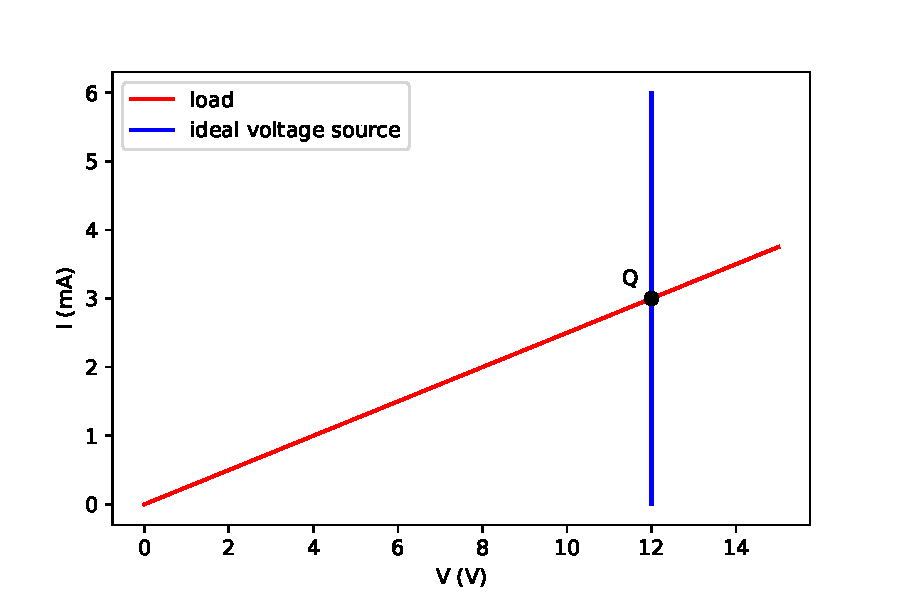
\includegraphics[height=0.3\textheight]{figs/thev_ideal.pdf} \\
\caption{ The source $I-V$ curve for an ideal $12~\rm V$ voltage source, and the load $I-V$ curve for a $4~\rm k\Omega$ resistor.   The operating point for the circuit when the load is connected to the source is the intersection of these two curves at point $Q$.  The power provided by the source and consumed by the load is the product $IV$ at the operating point.}
\label{fig:vr_iv}
\end{center}
\end{figure}

\begin{figure}[htbp]
\begin{center}
\begin{tabular}{cc}
\begin{circuitikz}[line width=1pt]
\draw (0,0) node[right]{A} to[short,o-] ++(-1.0,0) to[battery,bipoles/length=1.5cm,l=$V_1$] ++(0,+2.0) 
to[R, l=$R_{\rm src}$] ++(0,+2.0) to[short, i>=$I$,-o] ++(1.0,0) node[right]{B};
\draw (1, 0.0) to [open,v_>=$V$] (1,4.0);
\end{circuitikz} &
\begin{circuitikz}[line width=1pt]
\draw (0,0) node[left]{A} to[short,o-] ++(1.0,0) to[R,l=$R_1$] ++(0,+4.0) to[short, i<=$I$,-o] ++(-1.0,0) node[left]{B};
\end{circuitikz} \\
(a) & (b) \\
\end{tabular}
\caption{ Two terminal network diagrams (a) for a voltage source include source resistance $R_{src}$ as the source, and (b) a load resistor.}
\label{fig:vrr}
\end{center}
\end{figure}

\begin{figure}[htbp]
\begin{center}
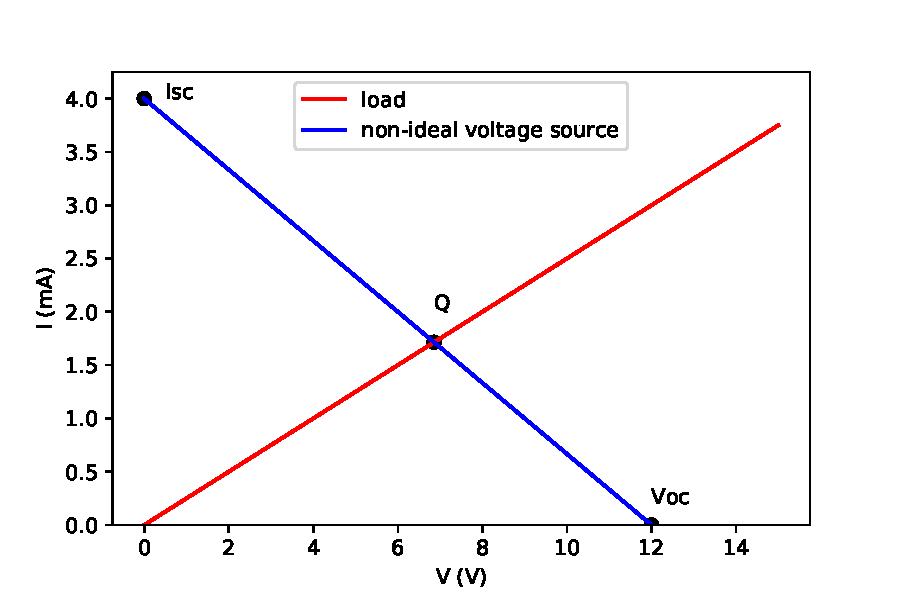
\includegraphics[height=0.3\textheight]{figs/thev_nonideal.pdf} \\
\caption{ $I-V$ curves for a non-ideal $12~\rm V$ source which includes a source resistance of $R_{\rm src} = 3~\rm k\Omega$ and a load resistance of $4~\rm k\Omega$.  The short-circuit current and open-circuit voltage, which fully constrain the line, are shown.  The intersection of the two curves at point $Q$ is the operating point of the circuit consisting of the source plus the load.}
\label{fig:vrr_iv}
\end{center}
\end{figure}

So far, we have only considered ideal voltage sources.  All real voltage sources have additional parasitic features.  For instance, real batteries provide a voltage but also have an internal resistance.  In fact all voltage source you will encounter in ordinary circuits will have some source resistance, which is modeled as an additional resistor in series with an ideal source, as shown in Fig.~\ref{fig:vrr}a.  What is the $I$-$V$ curve of such an object?  If you leave the two terminals isolated from each other (an open circuit) no current will flow, so the voltage drop across the resistor $R_{\rm src}$ is zero, and the voltage is simple $V = V_1$.
If you short circuit the terminals A and B, a current $I_{sc} = V_1 / R_{\rm src}$ will flow.  Ohm's Law ensures a linear relationship between I and V, so that these two points fully define the $I$-$V$ curve for this device, as shown in Fig.~\ref{fig:vrr_iv}.  It is left as an exercise to show that the slope of the source $IV$ curve in this case is $-1/R_{\rm src}$, in entirely reasonable result, since the slope of a load resistor $IV$ curve, with current in the opposite direction, is $1/R$.

\begin{figure}[htbp]
\begin{center}
 \begin{circuitikz} [american voltages, baseline=(current bounding box.center)]
    \ctikzset { label/align = straight }
    \draw (0,0)

    % fake resistor, using for voltage label only
    (3.5, 1.8) to [open,v=$V$] (3.5,0.2)

    (1.5,2) to[short, -o] (1.5,2)
    (1.5,2) to[short,i=$I$, -o] (5,2)
    to[short] (4.5,2)
    (1.5,0) to[short, -o] (1.5,0)
    (1.5,0) to[short, -o] (5,0)
    to[short] (4.5,0);
    \node[draw,minimum width=2cm,minimum height=2.4cm,anchor=south west] at (4.5,-0.2){Load};
    \node[draw,minimum width=2cm,minimum height=2.4cm,anchor=south west] at (0, -0.2){Source};
  \end{circuitikz}
\end{center}
\caption{A generic source and load.}
\label{fig:generic_source_load}
\end{figure}

No matter how complicated the actual circuit is, if one part is connected to the next by only two connections, the source and load analysis can be applied.  This is shown conceptually in Fig.~\ref{fig:generic_source_load}.  In fact, even if there are more than two connections, this analysis can be used if the additional connections have a negligible effect on the voltage and current that is under consideration.  Very often, the second connection is simply the common ground.  A very common arrangement for a complicated circuit is one that receives a signal and processes it in some way, e.g. amplifying it, before passing the output to the next stage, which further processes the signal, e.g. applying a filter, before passing it to the next stage.  When analyzing such a circuit, each stage is a load for the previous stage, and source for the next stage.

\section{Thevenin Equivalent Circuit}

There's a tremendously powerful tool that we get, essentially for free, from our understanding of $I-V$ curves for two-terminal networks.

If you set out to build the most complicated two-terminal network that you can imagine which includes resistors, voltages source, and wires, you have at your disposal:   Ohm's Law, Kirchoff's Laws, and the Superposition principle.  These are all linear equations, and so the source $I$-$V$ curve of your circuit, despite all your efforts, will always remain a straight line, such as that of Fig.~\ref{fig:thevenin_source}.  But we can construct any straight line we wish using only a single voltage source in series with a single resistor.  This means that any two-terminal network of resistors and voltage sources can be considered equivalently, with respect to those two-terminals, as a single voltage source in series with a single resistor.  An example is shown in Fig.~\ref{fig:thev_eg}.

Conceptually, we can imagine making two measurements of any two-terminal network to determine it's Thevenin equivalent.  Measuring the open-circuit voltage across terminals A and B reveals the Thevenin equivalent voltage $V_{\rm th}$.  Measuring the current $I_{\rm sc}$ that flows when we short-circuit terminals A and B allows us to determine $R_{\rm th}$ from:
\begin{displaymath}
V_{\rm th} = R_{\rm th} I_{\rm sc}.
\end{displaymath}

In practice, it's almost always easiest to make effective use of the superposition principle.  The Thevenin equivalent resistance is simply the equivalent resistance if all voltage sources are replaced with short-circuits.  If there are multiple voltage sources, it's usually easiest to consider only one voltage source at a time, setting all other voltage source to short-circuits.  The Thevenin equivalent voltage is then the sum of these partial solutions.

\begin{figure}[htbp]
\begin{center}
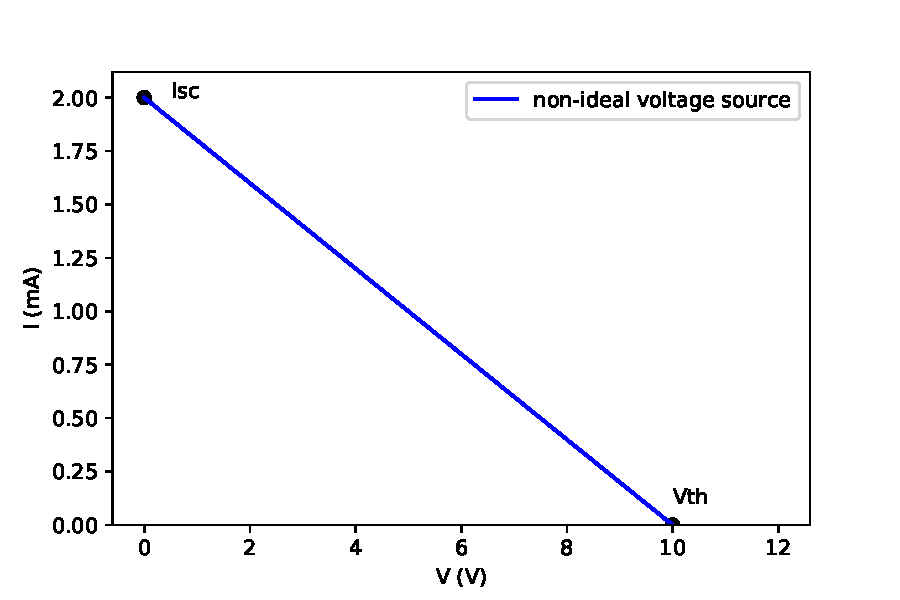
\includegraphics[height=0.3\textheight]{figs/thevenin.pdf} 
\caption{ The source IV curve for an arbitrary two terminal network.}
\label{fig:thevenin_source}
\end{center}
\end{figure}

\begin{figure}[htbp]
\begin{center}
\begin{tabular}{cc}
\begin{circuitikz}[line width=1pt]
\draw (0,0) node[right]{A} to[short,o-*] ++(-1.0,0) coordinate(X) to[resistor,l_=$R_8$] ++(0,2.0)
to[resistor,l_=$R_7$] ++(0,2.0) to[resistor,l_=$R_6$] ++(0,2.0) to[short,-o] ++(1.0,0) node[right]{B};
\draw (X) to[resistor,l=$R_5$] ++(-2.0,0) coordinate(X);
\draw (X) to[voltage source,bipoles/length=1.5cm,l=$V_1$] ++(0,+2.0) coordinate(X) to[resistor,l=$R_4$,*-*] ++(2.0,0);
\draw (X) to[voltage source,bipoles/length=1.5cm,l=$V_2$] ++(0,+2.0) coordinate(X) to[resistor,l=$R_3$,*-*] ++(2.0,0);
\draw (X) to[resistor,l=$R_1$] ++(0,+2.0) to[resistor,l=$R_2$,-*] ++(2.0,0);
\end{circuitikz} &
\begin{circuitikz}[line width=1pt]
\draw (0,0) node[right]{A} to[short,o-] ++(-1.0,0) to[voltage source,bipoles/length=1.5cm,l=$V_{\rm th}$] ++(0,+2.0) 
to[R, l=$R_{\rm th}$] ++(0,+2.0) to[short, i>=$I$,-o] ++(1.0,0) node[right]{B};
\end{circuitikz} \\
(a) & (b) \\
\end{tabular}
\caption{ Two-terminal network diagrams for (a) a fairly complicated network, and (b) it's Thevenin equivalent.}
\label{fig:thev_eg}
\end{center}
\end{figure}


\section{Exercises}

\begin{enumerate}

\item Derive Equations~\ref{eqn:rseries} and \ref{eqn:rparallel}.

\item Derive Equation~\ref{eqn:idivider}.

\item Show that the power consumed by a resistor of resistance $R$ conducting a current $I$ is:
\begin{displaymath}
P = I^2R
\end{displaymath}

\item Show that the power consumed by a resistor of resistance $R$ held at a voltage $V$ is:
\begin{displaymath}
P = V^2/R
\end{displaymath}

\item Using circuit analysis, determine the operating point (Q) of the
  circuit in Fig.~\ref{fig:vrr_iv} and compare with the value you read
  off from the plot.

%\item Draw the $IV$ curve for an ideal voltage source and a
%  short-circuit.  Do they intersect?  What do you suppose would happen
%  if you attempted to short-circuit an ideal voltage source?  Now draw
%  an open circuit ($I=0$).  What is the operating point of a voltage
%  source with it's terminals left open?  


\item We already discussed ideal voltage sources which will provide
  any necessary current to maintain a constant voltage across two
  terminals.  Another linear circuit element source is an ideal
  current source, which provides any necessary voltage to maintain a
  constant current through its two terminals.  Sketch the $IV$ curve
  for a constant voltage source and a constant current source.  Ideal
  voltage sources have zero intrinsic resistance.  What intrinsic
  resistance does an ideal current source have?  (Hint: look at the IV
  curve and recall the relationship between slope and resistance.)
  One way to make a current source is to place a very large resistor
  in series with a very large voltage source.  Is this consistent with
  your answer?

%\item Draw the $IV diagrams$ for an ideal current source and an open-circuit (I=0).  Do they intersect?  What do you suppose would happen if you attempted to leave the terminals of an ideal voltage source open?  Now draw a short circuit.  What is the operating point of a voltage source with it's terminals left open?  

\item Find the Thevenin Equivalent voltage, resistance, and short-circuit current for the following two terminal network:
\begin{center}
\begin{circuitikz}[line width=1pt]
\draw (0,0) node[right]{A} to[short,o-*] coordinate(X) ++(-1.0,0) coordinate(X) to[resistor,l_=$R_2$] ++(0,2.0) to[short,*-o] ++(1.0,0) node[right]{B};
\draw (X) to[short,*-] ++ (-2.0,0) to[voltage source,bipoles/length=1.5cm,l=$V_1$] ++(0,+2.0) to[resistor,l=$R_1$] ++(2.0,0);
\end{circuitikz} \\
\end{center}
Leave your answer in terms of $R_1$, $R_2$, and $V_1$.

\item Find the Thevenin Equivalent voltage and resistance for the following two-terminal network:
\begin{center}
\begin{circuitikz}[line width=1pt]
\draw (0,0) node[right]{A} to[short,o-] ++(-1.0,0) coordinate(X) 
to[voltage source,bipoles/length=1.5cm,l=$V_3$] ++(0,2.0) to[R,l=$R_3$] ++(0,2.0) 
to[short,-o] ++(1.0,0) node[right]{B};
\draw (X) to[short,*-] ++(-2.0,0) coordinate(X) 
to[voltage source,bipoles/length=1.5cm,l=$V_2$] ++(0,2.0) to[R,l=$R_2$] ++(0,2.0) 
to[short,-*] ++(2.0,0);
\draw (X) to[short,*-] ++(-2.0,0) coordinate(X) 
to[voltage source,bipoles/length=1.5cm,l=$V_1$] ++(0,2.0) to[R,l=$R_1$] ++(0,2.0) 
to[short,-*] ++(2.0,0);
\end{circuitikz} \\
\end{center}
Leave your answer in terms of $R_1$, $R_2$, $R_3$, $V_1$, $V_2$ and $V_3$.  

\item  When you ask why they are late with their share of the rent (again), your roommate explains that they would like to invest the money into buying inexpensive force sensors for about \$10 each.  They think they can use these to make cheap electronic drum kits and sell them at a profit.   The idea is to connect a force sensor acting as a switch between a $9~\rm V$ battery and an old $50~\rm \Omega$ (load resistance) speaker.  Each customer will supply their own battery and speaker, and the wire will be pilfered from Physics 80 lab.  While perusing the specs for the force sensor, you notice that they have a typical source resistance of about $100~\rm k\Omega$.    Model the proposal as a DC voltage divider, which is sufficient analysis to see what a terrible design your roommate has concocted.  What's the maximum voltage you would see across the speaker given the source resistance and load resistance?  What's the maximum power that would be consumed by the speaker?  Compare this with the power consumed by the speaker at typical operating voltages of at least $1~\rm V$.   Whatever you do, do not leave the room without the rent money in cash!!!

\end{enumerate}

\chapter{Alternating Current Circuits and Impedance}

\section{Resistors, Capacitors, and Inductors}

\begin{figure}[htbp]
\begin{center}
\begin{tabular}{ccc}
\begin{circuitikz}[line width=1pt]
\draw (0,0) node[left]{A} to[short,o-] ++(1.0,0) to[R,l=$R$] ++(0,+4.0) to[short, i<=$I$,-o] ++(-1.0,0) node[left]{B};
\draw (0,-1) node[]{$V_{AB} = IR$};
\end{circuitikz} &
\begin{circuitikz}[line width=1pt]
\draw (0,0) node[left]{A} to[short,o-] ++(1.0,0) to[C,l=$C$] ++(0,+4.0) to[short, i<=$I$,-o] ++(-1.0,0) node[left]{B};
\draw (1.7,2.4) node[left]{$Q$};
\draw (0,-1) node[]{$V_{AB} = \frac{Q}{C}$};
\end{circuitikz} &
\begin{circuitikz}[line width=1pt]
\draw (0,0) node[left]{A} to[short,o-] ++(1.0,0) to[L,l=$L$] ++(0,+4.0) to[short, i<=$I$,-o] ++(-1.0,0) node[left]{B};
\draw (0,-1) node[]{$V_{AB} = L \frac{dI}{dt}$};
\end{circuitikz} \\
(a) & (b) & (c) \\
\end{tabular}
\caption{The voltage across a (a) resistor, (b) capacitor, and (c) inductor.  The sign convention for all of these relationships implies that the component is being treated as a load, with current $I$ entering the positive terminal.  The charge $Q$ is the charge which builds up on the upper plate, while the lower plate will have charge $-Q$.}
\label{fig:rlc}
\end{center}
\end{figure}

We've already encountered our first two terminal electrical component, the resistor, which obeys Ohm's law.  When considering the sign of Ohm's law, one must remember that the definition implies that the resistor is being considered  as a load, as shown in Fig.~\ref{fig:rlc}a, with positive current directed into the positive terminal defining the voltage drop across the component.

A capacitor is a two terminal electrical component which stores energy in an electric field.  The electric field is the result of a build up of charge, positive on one terminal of the capacitor and negative on the other, which produces the electric field.  When considered as a load, with charge $Q$ on the upper terminal (and charge $-Q$ on the lower terminal) the voltage across a capacitor is:
\begin{displaymath}
V = \frac{Q}{C}
\end{displaymath}

An inductor is a two terminal electrical component which stores energy in a magnetic field when an electrical current passes through it.  Because of the property of self-inductance, an inductor tends to resist changes in current.  When considered as a load, the voltage across an inductor is:
\begin{displaymath}
V = L\frac{dI}{dt}
\end{displaymath}

While the capacitor and the inductor have the capability to store energy, none of these three components are capable of adding power to a circuit, and are therefore called passive components.

\section{Time dependence of a Capacitive Circuit}

\begin{figure}[htbp]
\begin{center}
\begin{circuitikz}[line width=1pt]
\draw (0,0) node[right]{A} to[short,o-*] coordinate(X) ++(-1.0,0) coordinate(X) to[C,l=$C$,i<=$I(t)$] ++(0,4.0) to[short,-o] ++(1.0,0) node[right]{B};
\draw (X) to[short,*-] ++ (-2.0,0) to[voltage source,bipoles/length=1.5cm,l=$V_0$] ++(0,+2.0)
to[cspst, bipoles/length=2.0cm] ++(0,2.0) to[resistor,l=$R$] ++(2.0,0);
\draw (-1.0,2.3) node[right]{$Q(t)$};
\end{circuitikz} 
\caption{Circuit for considering the behavior of a capacitor.}
\label{fig:rc}
\end{center}
\end{figure}

Consider the $RC$ circuit of Fig.~\ref{fig:rc} with the switch closed.  From KVL:
\begin{displaymath}
0 = V_0 - IR - \frac{Q}{C}
\end{displaymath}
or matching source voltage to load voltage:
\begin{displaymath}
V_0 = IR + \frac{Q}{C}
\end{displaymath}
The charge as a function of time $Q(t)$ therefore obeys the differential equation:
\begin{equation} \label{eqn:icap}
V_0 = \frac{dQ}{dt}R + \frac{Q(t)}{C}
\end{equation}
Our physical intuition leads us to try first for a steady-state solution of the form $Q(t) = Q_{\rm F}$ for some constant $Q_{\rm F}$, so that:
\begin{displaymath}
\frac{dQ}{dt} = 0
\end{displaymath}
and so Equation~\ref{eqn:icap} leads to:
\begin{displaymath}
Q_{\rm F} = C V_0.
\end{displaymath}
After enough time, the capacitor will charge to $CV_0$, the voltage across the capacitor will be equal to the applied voltage $V_0$, and so no current flow.  This is the steady-state behavior for this circuit.

However, imagine that at time $t=0$, the capacitor is initially uncharged with $Q=0$.  How will the circuit reach the steady-state?  Since the differential equation is linear, any solution to the homogenous version  (obtained by setting $V_0=0$):
\begin{equation} \label{eqn:hcap}
0 = \frac{dQ}{dt}R + \frac{Q(t)}{C}
\end{equation}
can be added to the steady-state solution to provide a solution to the non-homogenous version (with $V \ne 0$).  Differential equations which relate the rate of change of a quantity to the quantity itself invariably lead to the exponential function, and we are led to try:
\begin{displaymath}
Q(t) = A \exp(B t)
\end{displaymath}
for constants $A$ and $B$.  Applying Equation~\ref{eqn:hcap} leads to:
\begin{eqnarray*}
0 &=& R B A \, \exp(B t)  + \frac{Q(t)}{C}\\
0 &=& \left( RB + \frac{1}{C}\right) Q(t)
\end{eqnarray*}
which will be true provided that:
\begin{displaymath}
B = -\frac{1}{RC}
\end{displaymath}
That is solutions of the form:
\begin{displaymath}
Q(t) = A \, \exp(- t/\tau)
\end{displaymath}
with $\tau = RC$ satisfy Equation~\ref{eqn:hcap} and can be added to the steady state solution to obtain:
\begin{displaymath}
Q(t) = CV + A \, \exp(- t / \tau)
\end{displaymath}
which is the general solution to Equation~\ref{eqn:icap}.  (You can confirm this for yourself if this is the first time you have seen this approach used.)

For the specific case that $Q(0) = 0$, we conclude that $A = -CV$ and so:
\begin{displaymath}
Q(t) = CV_0 \left(1 - \exp(- t / \tau) \right)
\end{displaymath}
which describes a capacitor charging with a time constant $\tau = RC$ asymptotically approaching the steady-state $Q = CV_0$.  If follows that the voltage across the capacitor as a function of time is:
\begin{displaymath}
V(t) = \frac{Q(t)}{C} = V_0 \left(1 - \exp(- t / \tau) \right)
\end{displaymath}
while the current as a function of time is:
\begin{displaymath}
I(t) = \frac{dQ}{dt} = \frac{V_0}{R} \exp(- t / \tau) 
\end{displaymath}

The voltage and current as function of time for a charging capacitor is shown in Fig.~\ref{fig:vit_trans}
Notice that at $t=0$, we have simply $I = V_0/R$, as there is no voltage across the capacitor while $Q=0$.

\begin{figure}[htbp]
\begin{center}
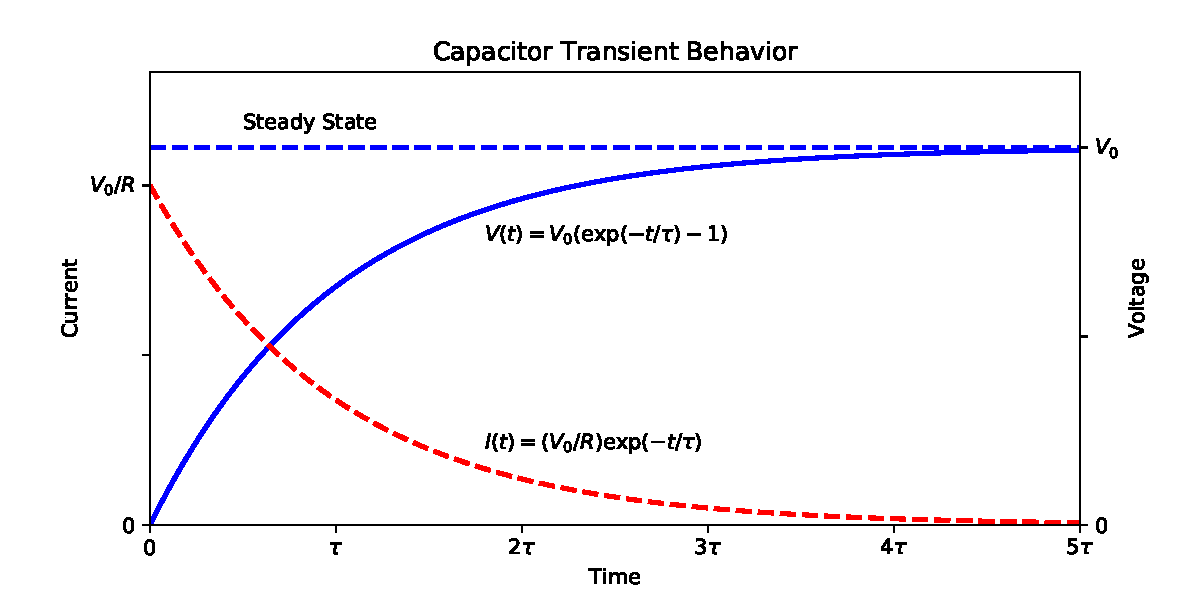
\includegraphics[height=0.3\textheight]{figs/transient_cap.pdf} \\
\caption{Current and voltage across a charging capacitor as a function of time.}
\label{fig:vit_trans}
\end{center}
\end{figure}

\section{Time dependence of an Inductive Circuit}

\begin{figure}[htbp]
\begin{center}
\begin{circuitikz}[line width=1pt]
\draw (0,0) node[right]{A} to[short,o-*] coordinate(X) ++(-1.0,0) coordinate(X) to[L,l=$L$,i<=$I$] ++(0,4.0) to[short,-o] ++(1.0,0) node[right]{B};
\draw (X) to[short,*-] ++ (-2.0,0) to[voltage source,bipoles/length=1.5cm,l=$V_0$] ++(0,+2.0)
to[cspst, bipoles/length=2.0cm] ++(0,2.0) to[resistor,l=$R$] ++(2.0,0);
\end{circuitikz} 
\caption{\label{fig:rl} Circuit for considering the behavior of an inductor.}
\end{center}
\end{figure}

Consider the $RL$ circuit of Fig.~\ref{fig:rl} with the switch closed.  From KVL:
\begin{displaymath}
0 = V_0 - IR - L\frac{dI}{dt}
\end{displaymath}
or matching source voltage to load voltage:
\begin{displaymath}
V_0 = IR + L\frac{dI}{dt}
\end{displaymath}
The current as a function of time $I(t)$ therefore obeys the differential equation:
\begin{equation} 
V_0 = R I(t) + L \frac{dI}{dt}
\end{equation}
It is left as an exercise to show that the steady-state solution is the constant current:
\begin{equation} \label{eqn:inductorss}
I = V_0 / R
\end{equation}
and the general solution is 
\begin{equation} \label{eqn:inductorgen}
I(t) = (V_0 / R) + A \, \exp(-t/\tau) 
\end{equation}
with $\tau = L / R$.

For the specific case that $I(0) = 0$, we conclude that $A = -V/R$ and so:
\begin{displaymath}
I(t) = (V_0/R) \, (1 - \exp(-t / \tau)).
\end{displaymath}
Notice that at $t=0$, we have simply $I = V_0/R$, as there is no voltage across the capacitor while $Q=0$.

\section{Alternating Current}
 
 We've seen now that voltages can be a function of time $V(t)$.    If the steady-state voltage levels in a circuit are constant with time, it is referred to as a direct current (DC) circuit, because the currents that result tend to flow in the same direction.   A circuit with a time-dependence which averages to zero by oscillating back and forth is referred to as an alternating current (AC).   If the voltage is changing with time, but does not average to zero, the signal is a mixture of AC and DC.  The DC contribution is the average value, and the AC component is what remains when this DC component is removed.  We will use a convention that lower-case variables, such as $v$ and $i$ refer to AC quantities, and upper case variables, such as $V$ and $I$ refer to DC quantities.  Transients responses, which are often ignored in AC and DC circuit analysis, will remain as time-dependent upper case variables, such as $V(t)$ and $I(t)$.
   
 Of particular importance, is a sinusoidal voltage of the form:
 \begin{displaymath}
 v(t) = v_{\rm p} \cos(\omega t + \phi).
 \end{displaymath}
 The parameter $v_p$ in this equation is called the peak AC voltage.  The parameter $\omega$ is the angular frequency, related to the frequency $f$ by $\omega = 2 \pi f$.  The parameter $\phi$ determines the phase of the voltage.

Other common measurements of the AC voltage level are the peak-to-peak AC voltage, which for a pure sine wave is:
\begin{displaymath}
v_{\rm pp} = 2 v_{\rm p}.
\end{displaymath}
And the root-mean-square (RMS) average AC voltage:
\begin{displaymath}
v_{\rm rms} = \sqrt{\langle v^2(t) \rangle}
\end{displaymath}
where $\langle f(t) \rangle$ denotes the time average:
\begin{displaymath}
\langle f(t) \rangle \equiv \frac{1}{T}\int_{-T/2}^{T/2} f(t)
\end{displaymath}
It is left as an exercise to show that for a pure sine wave:
\begin{displaymath}
v_{\rm rms} = v_{\rm p} / \sqrt{2}
\end{displaymath}
When left unspecified, an AC voltage usually refers to an RMS voltage.  So when we refer to a $120~\rm V$ household outlet, we mean specifically a $120~\rm V$~(AC) RMS voltage.  

Understanding the response of circuits to AC voltages is of paramount importance.  This is not just because our power arrives as an AC voltage.  Much of modern electronics, both at home and in the lab, is used for signal processing of time dependent signals encoded as $V(t)$.  Fourier's Theorem informs us that any time-dependent signal can be interpreted as a sum of sine and cosine functions of different frequencies.  So if we can understand the response of our circuit to DC plus AC sine waves of any frequency, we know everything there is to know about the circuit.

\section{Passive Components and Alternating Current}

\begin{figure}[htbp]
\begin{center}
\begin{circuitikz}[line width=1pt]
\draw (0,0) coordinate(X) to[sinusoidal voltage source,bipoles/length=1.5cm] ++(0,+2.0) 
to [short,i=$i$] ++(1.5,0) to[R,l_=$R$] ++(0,-2.0) to[short] ++(-1.5,0);
\draw (X) node[ground,yscale=2.0]{};
\draw (0.0,1.7) node[left]{$v(t)$};
\end{circuitikz} 
\caption{An AC voltage source applied to a resistor.}
\label{fig:acr}
\end{center}
\end{figure}

We are now ready to consider what happens to resistors, capacitors, and inductors when an AC voltage is applied across them.  We'll start with the easiest case, the resistor, and the circuit illustrated in Fig.~\ref{fig:acr}.  We've introduced a new symbol, the AC voltage source.  We'll adopt the convention that the positive terminal is always at the top.  We'll also reference the negative terminal to ground, because the function generator you use in lab is referenced to ground.  To reinforce the convention that the positive terminal is at the top, that is where we will label the time dependent voltage provided, which we will take in most cases as:
\begin{displaymath}
v(t) = v_{\rm p} \cos(\omega t).
\end{displaymath}
In the case of the resistor, Ohm's law informs us immediately that:
\begin{displaymath}
i(t) = v(t) / R = (1/R) \, v_{\rm p} \cos(\omega t)
\end{displaymath}
If we are only concerned with the RMS current and voltage, we find:
\begin{displaymath}
v_{\rm rms}/i_{\rm rms} = R 
\end{displaymath}
Ohm's law is alive and well for AC circuits!

\begin{figure}[htbp]
\begin{center}
\begin{circuitikz}[line width=1pt]
\draw (0,0) coordinate(X) to[sinusoidal voltage source,bipoles/length=1.5cm] ++(0,+2.0) 
to [short,i=$i$] ++(1.5,0) to[C,l_=$C$] ++(0,-2.0) to[short] ++(-1.5,0);
\draw (X) node[ground,yscale=2.0]{};
\draw (0.0,1.7) node[left]{$v(t)$};
\end{circuitikz} 
\caption{An AC voltage source applied to a capacitor.}
\label{fig:acr}
\end{center}
\end{figure}

The capacitance relates the voltage to the charge on the capacitor:
\begin{displaymath}
q(t)  = C v(t)
\end{displaymath}
and so taking the derivative with respect to time:
\begin{displaymath}
i = \frac{dq}{dt} = C \frac{dv}{dt}
\end{displaymath}
So in this case, with $v(t) = v_p \cos(\omega t)$
\begin{eqnarray*}
i &=& C (-\omega v_p \sin(\omega t))\\
 &=& (\omega C) v_p \cos \left( \omega t + \frac{\pi}{2} \right) \\
\end{eqnarray*}
The RMS values are related by:
\begin{displaymath}
v_{\rm rms}/i_{\rm rms} = \frac{1}{\omega C}
\end{displaymath}
but the phase of the voltage relative to the current is $\Delta \phi = -\pi/2$ (due to the $+\pi/2$ term in the current.)

\begin{figure}[htbp]
\begin{center}
\begin{circuitikz}[line width=1pt]
\draw (0,0) coordinate(X) to[sinusoidal voltage source,bipoles/length=1.5cm] ++(0,+2.0) 
to [short,i=$i$] ++(1.5,0) to[L,l_=$L$] ++(0,-2.0) to[short] ++(-1.5,0);
\draw (X) node[ground,yscale=2.0]{};
\draw (0.0,1.7) node[left]{$v(t)$};
\end{circuitikz} 
\caption{An AC voltage source applied to a inductor.}
\label{fig:acr}
\end{center}
\end{figure}

The inductance relates the voltage to the rate of change of the current:
\begin{displaymath}
\frac{di}{dt}  =\frac{1}{L} v(t)
\end{displaymath}
and so integrating with respect to time:
\begin{displaymath}
i = \frac{1}{L} \int dt \; v(t) 
\end{displaymath}
So in this case, with $v(t) = v_p \cos(\omega t)$
\begin{eqnarray*}
i &=& \frac{1}{L}  \int dt \; v_p \cos(\omega t)\\ 
&=& \frac{1}{L} \left( \frac{v_p}{\omega} \sin(\omega t) \right) + I_0\\
&=& \frac{1}{\omega L} \cos \left( \omega t - \frac{\pi}{2} \right)  + I_0\\
\end{eqnarray*}
The constant of integration $I_0$ is a constant direct current.  Indeed, with no resistance in this idealized circuit, a DC current could flow indefinitely, with no DC voltage drop anywhere in the circuit.  Of course, in a real circuit with resistance, such a current would quickly disappear.  We'll simply assume $I_0=0$ for our purpose of understanding the AC response, and so:
\begin{eqnarray*}
i &=& \frac{1}{\omega L} \cos \left( \omega t - \frac{\pi}{2} \right)\\
\end{eqnarray*}
The RMS values are related by:
\begin{displaymath}
v_{\rm rms}/i_{\rm rms} = \omega L
\end{displaymath}
but the phase of the voltage relative to the current is $\Delta \phi = \pi/2$ (due to the $-\pi/2$ term in the current.)

\begin{figure}[htbp]
\begin{center}
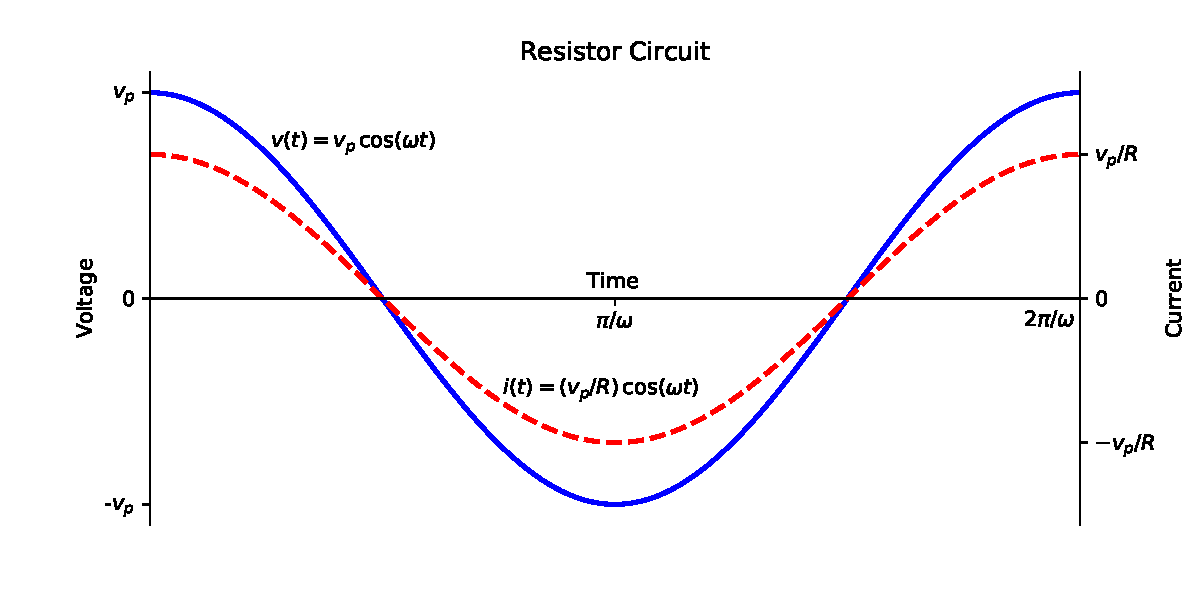
\includegraphics[height=0.3\textheight]{figs/vit_res.pdf} \\
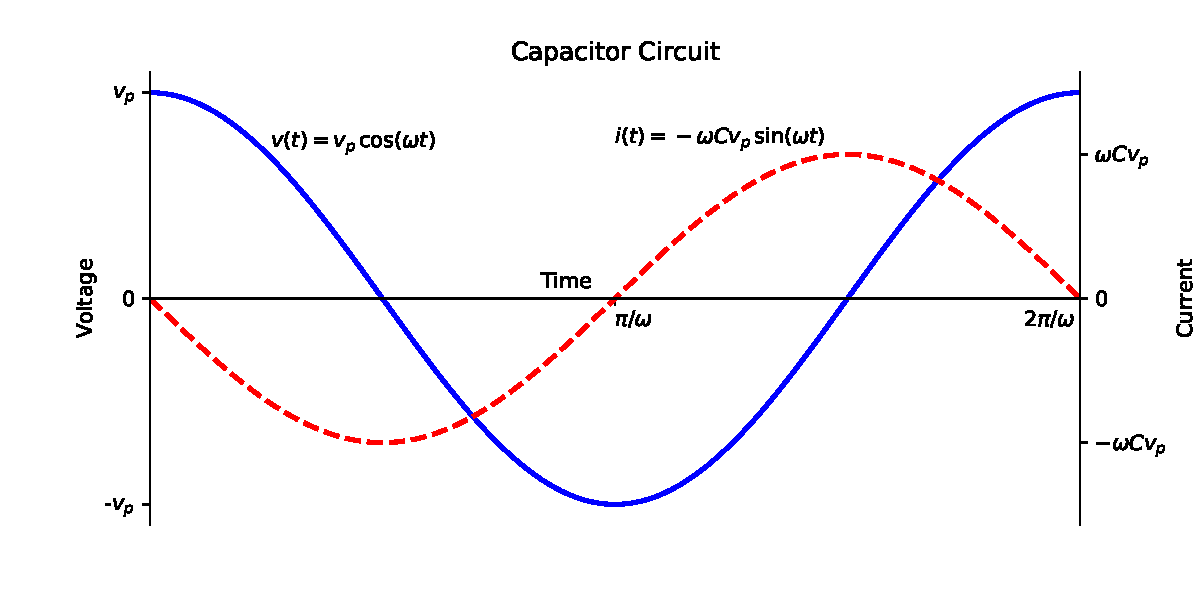
\includegraphics[height=0.3\textheight]{figs/vit_cap.pdf} \\
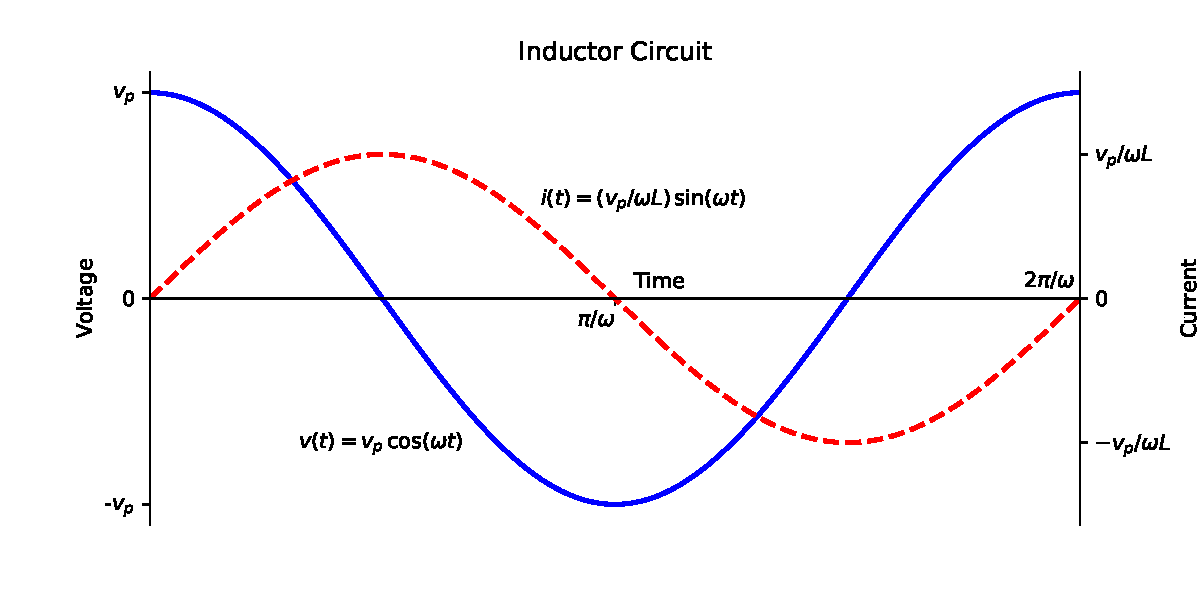
\includegraphics[height=0.3\textheight]{figs/vit_ind.pdf} \\
\caption{ Time dependence of AC voltage and current in a resistor, capacitor, or inductor.}
\label{fig:vit}
\end{center}
\end{figure}



\begin{table}
\caption{Summary or relationship between current and voltage for AC signals.}
\label{tbl:rmsimp}
\begin{center}
\begin{tabular}{lrr}
component & $v_{\rm rms} / i_{\rm rms} $ & $\Delta \phi$ \\
\hline
\\
resistor ($R$) & $R$ & $0$ \\
\\
capacitor ($C$) & $\displaystyle \frac{1}{\omega C}$ & $\displaystyle -\frac{\pi}{2}$ \\
\\
inductor ($L$) & $\omega L$ & $\displaystyle +\frac{\pi}{2}$ \\
\\
\end{tabular}
\end{center}
\end{table}

The present situation is summarized in Table~\ref{tbl:rmsimp} and Fig.~\ref{fig:vit}, and it is tempting to think we are finished.  After all, we've found an Ohm's Law like relationship between $v_{\rm rms}$ and $i_{\rm rms}$ for capacitors and inductors, so shouldn't we able to analyze AC circuits just like DC circuits?  The problem is that we do not yet have an equivalent for Kirchoff's Laws.  DC voltages and currents simply add, but now our voltages have a phase, so we can't, for instance, simply add RMS voltages.  Faced with a more complicated circuit, we could derive a new, more complicated differential equation, and solve that.  Fortunately, there's an easier way!

\section{Phasors}

\begin{figure}[htbp]
\begin{center}
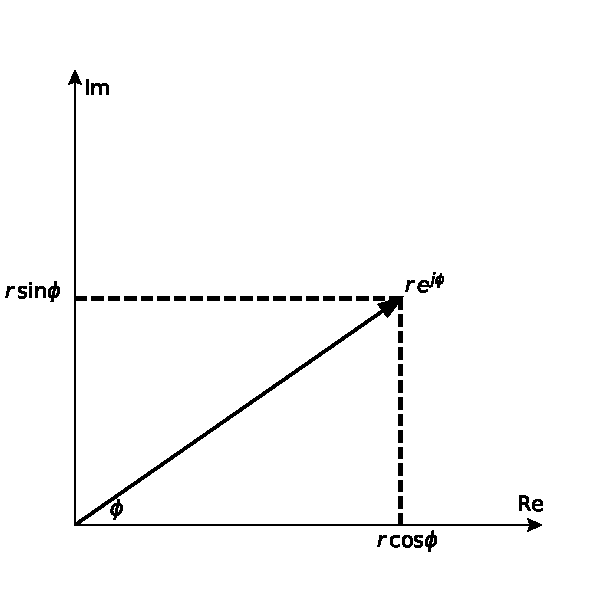
\includegraphics[height=0.3\textheight]{figs/complex.pdf} \\
\caption{ The geometry of the complex plane.}
\label{fig:complex}
\end{center}
\end{figure}

Recall Euler's Formula, which Feynman called ``our jewel'':
\begin{displaymath}
e^{j\phi} = \cos \phi + j \sin \phi 
\end{displaymath}
where we will use $j$ as the unit imaginary number, to avoid confusion with the AC current $i$.  This result has a beautiful geometric interpretation that allows us to consider the real and imaginary parts of a complex number as two components of a vector which has a magnitude and phase.  In particular, we can relate the cosine function to the real part of an imaginary number:
\begin{displaymath}
r \cos \phi = \Re \{ r e^{j\phi} \}. 
\end{displaymath}
We can therefore consider any AC signal:
\begin{displaymath}
v(t) = v_{\rm p} \cos ( \omega t + \phi)
\end{displaymath}
to be the real part of a time-dependent complex number:
\begin{displaymath}
v(t) = \Re \{ v_{\rm p} \exp ( j (\omega t + \phi))\}.
\end{displaymath}
We can rearrange this complex number as:
\begin{eqnarray*}
v(t) &=& \Re \{ v_{\rm p} e^{j\phi} \cdot e^{j \omega t} \} \\
&=& \Re \{ \tilde{v} \cdot e^{j \omega t} \} \\
\end{eqnarray*}
where we have defined the quantity:
\begin{equation}
\tilde{v} \equiv v_{\rm p} e^{j \phi}
\label{eqn:phasor}
\end{equation}

which we call a phase vector or simply phasor.  The phasor is a complex number that contains the magnitude and phase information for the particular AC signal we are considering.  It is simply a complex number, with no time dependence.  The time-dependent part of the entire expression comes from the term $e^{j \omega t}$, and is the same for every AC signal of frequency $\omega$.  Once we have specified the frequency of an AC circuit, there is a one-to-one corresponds with time dependent functions like v(t), and the phasor.  The phasor for an AC signal $v(t) = v_{\rm p} cos(\omega t + \phi)$ is given by the definition in Equation~\ref{eqn:phasor}.  To obtain the time-dependent signal from a phasor we simply calculate:
\begin{equation}
v(t) = \Re \{ \tilde{v} e^{j \omega t} \}
\end{equation}

\section{Impedance}

\begin{figure}[htbp]
\begin{center}
\begin{tabular}{ccc}
\begin{circuitikz}[line width=1pt]
\draw (0,0) coordinate(X) to[sinusoidal voltage source,bipoles/length=1.5cm] ++(0,+2.0) 
to [short,i=$\tilde{i}$] ++(1.5,0) to[R,l_=$R$] ++(0,-2.0) to[short] ++(-1.5,0);
\draw (X) node[ground,yscale=2.0]{};
\draw (0.0,1.7) node[left]{$\tilde{v}$};
\end{circuitikz} &
\begin{circuitikz}[line width=1pt]
\draw (0,0) coordinate(X) to[sinusoidal voltage source,bipoles/length=1.5cm] ++(0,+2.0) 
to [short,i=$\tilde{i}$] ++(1.5,0) to[C,l_=$C$] ++(0,-2.0) to[short] ++(-1.5,0);
\draw (X) node[ground,yscale=2.0]{};
\draw (0.0,1.7) node[left]{$\tilde{v}$};
\end{circuitikz} &
\begin{circuitikz}[line width=1pt]
\draw (0,0) coordinate(X) to[sinusoidal voltage source,bipoles/length=1.5cm] ++(0,+2.0) 
to [short,i=$\tilde{i}$] ++(1.5,0) to[L,l_=$L$] ++(0,-2.0) to[short] ++(-1.5,0);
\draw (X) node[ground,yscale=2.0]{};
\draw (0.0,1.7) node[left]{$\tilde{v}$};
\end{circuitikz} \\
(a) & (b) & (c) \\
\end{tabular}
\caption{An AC voltage source applied to (a) a resistor, (b) a capacitor, and (c) an inductor.}
\label{fig:aclcr}
\end{center}
\end{figure}

For a resistor driven by a sinusoidal voltage source as in Fig.~\ref{fig:aclcr}a, Ohm's law states that:
\begin{displaymath}
i(t) = v(t) / R 
\end{displaymath}
If we write v(t) in terms of its associated phasor $\tilde{v}$:
\begin{eqnarray*}
i(t) &=& \frac{\Re \{ \tilde{v} \; e^{j \omega t}\}}{R} \\
&=& \Re \left\{ \frac{\tilde{v}}{R} \; e^{j \omega t} \right\} \\
\end{eqnarray*}
we can see that $i(t)$ is itself associated with the phasor:
\begin{displaymath}
\tilde{i} = \frac{\tilde{v}}{R}
\end{displaymath}
and so there is an Ohm's Law relationship between the phasors:
\begin{displaymath}
\tilde{v} = R \; \tilde{i}
\end{displaymath}

For a capacitor driven by a sinusoidal voltage source as in Fig.~\ref{fig:aclcr}b, we showed above that the current is related to the derivative of the voltage:
\begin{displaymath}
i(t) = C \, \frac{dv}{dt}
\end{displaymath}
If we write v(t) in terms of its associated phasor $\tilde{v}$:
\begin{eqnarray*}
i(t) &=& C \, \frac{d}{dt} \, \Re \{ \tilde{v} \; e^{j \omega t}\} \\
&=& \Re \left\{ \tilde{v} C \frac{d}{dt} \; e^{j \omega t} \right\} \\
&=& \Re \left\{ \tilde{v} j \omega C \; e^{j \omega t} \right\} \\
\end{eqnarray*}
where in the last step we have used the fact that:
\begin{displaymath}
\frac{d}{dt} e^{\alpha t} = \alpha e^{\alpha t}.
\end{displaymath}
From:
\begin{eqnarray*}
i(t) &=& \Re \left\{ \tilde{v} j \omega C \; e^{j \omega t} \right\} \\
\end{eqnarray*}
we can see that $i(t)$ is associated with the phasor:
\begin{displaymath}
\tilde{i} = j \omega C \tilde{v}
\end{displaymath}
which we can think of as Ohm's Law for a capacitor:
\begin{displaymath}
\tilde{v} = \frac{1}{j \omega C} \tilde{i}
\end{displaymath}
It's worth taking a moment to marvel over what we have accomplished here:  we replaced the differential equation describing the relations between $v(t)$ and $i(t)$ with mere multiplication of a phasor by a complex number.  We can analyze circuits simply according to the phasors, and convert our answer to time dependent signals whenever needed.  We already knew that the magnitude of the voltage and current were simply related.  By using phasors, one complex number describes the change in magnitude and the change in phase.

Now let's turn to the inductor, driven by a sinusoidal voltage source as in Fig.~\ref{fig:aclcr}c, for which we already determined that current is related to the integral of the voltage:
\begin{displaymath}
i = \frac{1}{L} \int dt \; v(t) 
\end{displaymath}
It is left as an exercise to show that the phasors for current and voltage are related by:
\begin{displaymath}
\tilde{v} = j \omega L \tilde{i}.
\end{displaymath}

\begin{table}
\caption{Impedances of passive-components}
\label{tbl:impedance}
\begin{center}
\begin{tabular}{ccc}
Component & Impedance & $\Delta \phi$ \\
\hline
\\
$R$ & $R$ & 0 \\
\\
$C$ & $\displaystyle \frac{1}{j \omega C}$ & $\displaystyle -\frac{\pi}{2}$ \\
\\
$L$ & $j \omega L$ & $\displaystyle +\frac{\pi}{2}$ \\

\end{tabular}
\end{center}
\end{table}

We've now shown that for all three of our passive components ($R$, $C$, and $L$) the phasor for voltage is simply the product of the phasor for the current times a complex number, which we call the impedance, $Z$.  We call the imaginary part of the impedance the reactance $X$, and the real part the resistance:
\begin{eqnarray*}
({\rm impedance}) &=& ({\rm resistance}) + j ({\rm reactance} ) \\
Z &=& R + j X \\
\end{eqnarray*}
These results are summarized in Table~\ref{tbl:impedance}.  

Kirchhoff's Voltage Laws and Kirchhoff's Current Law continue to hold for the time dependent voltages and currents, but they apply equally to the (constant valued) complex phasors.  A new Ohm's Law, which applies to all passive components states that:
\begin{displaymath}
\tilde{v} = Z \tilde{i}
\end{displaymath}
All of our previous results therefore apply with resistance replaced by impedance.  In particular, the impedance of components in series adds linearly:
\begin{equation} \label{eqn:zseries}
Z_{\rm eq} = \sum_i Z_i. 
\end{equation}
whereas for components in parallel:
\begin{equation} \label{eqn:zseries}
\frac{1}{Z_{\rm eq}} = \sum_i \frac{1}{Z_i}. 
\end{equation}




\section{Passive Filters}

\begin{figure}[htbp]
\begin{center}
\begin{tabular}{cc}
\begin{circuitikz}[line width=1pt]
\draw (0,0) node[ground,yscale=2.0]{} to[sinusoidal voltage source,bipoles/length=1.5cm] ++(0,+4.0) 
to [short,i=$\tilde{i}$] ++(1.5,0) to[R,l_=$R$] ++(0,-2.0) coordinate(B)
to[C,l_=$C$] ++(0,-2.0) coordinate(A) to[short] ++(-1.5,0);
\draw (0.0,2.75) node[left]{$\tilde{v}_{\rm in}$};
\draw (B) to[short,*-o] ++(1.5,0) node[right]{$\tilde{v}_{\rm out}$};
\end{circuitikz} &
\begin{circuitikz}[line width=1pt]
\draw (0,0) node[ground,yscale=2.0]{} to[sinusoidal voltage source,bipoles/length=1.5cm] ++(0,+4.0) 
to [short,i=$\tilde{i}$] ++(1.5,0) to[C,l_=$C$] ++(0,-2.0) coordinate(B)
to[R,l_=$R$] ++(0,-2.0) coordinate(A) to[short] ++(-1.5,0);
\draw (0.0,2.75) node[left]{$\tilde{v}_{\rm in}$};
\draw (B) to[short,*-o] ++(1.5,0) node[right]{$\tilde{v}_{\rm out}$};
\end{circuitikz} \\
(a) & (b) \\
\end{tabular}
\caption{Passive $RC$ (a) low-pass, and (b) high-pass filters.  Note that $\tilde{v}_{\rm in}$ and $\tilde{v}_{\rm out}$ are phasors corresponding to AC voltages referenced to ground.}
\label{fig:rcfilters}
\end{center}
\end{figure}

Consider the low-pass filter of Fig.~\ref{fig:rcfilters}a.   The output voltage $v_{\rm out}$ is simply the output of a voltage divider, but with the complex impedance taking the place of the resistance:
\begin{displaymath}
\tilde{v}_{\rm out} = \tilde{v}_{\rm in} \frac{Z_C}{Z_R + Z_C}
\end{displaymath}
And inserting the impedance of each device in terms of $R$ and $C$:
\begin{eqnarray*}
\tilde{v}_{\rm out} &=& \tilde{v}_{\rm in} \, \frac{\frac{1}{j \omega C}}{R + \frac{1}{j \omega C}}\\
&=& \tilde{v}_{\rm in} \, \frac{1}{1 + j \omega/\omega_0}\\
\end{eqnarray*}
Where we have defined the corner angular frequency: 
\begin{equation*}
\omega_0 = \frac{1}{RC}
\end{equation*}  
with corresponding corner frequency:
\begin{equation*}
f_0  \equiv \frac{\omega_0}{2\pi} = \frac{1}{2 \pi RC}.
\end{equation*}  
\begin{figure}[htbp]
\begin{center}
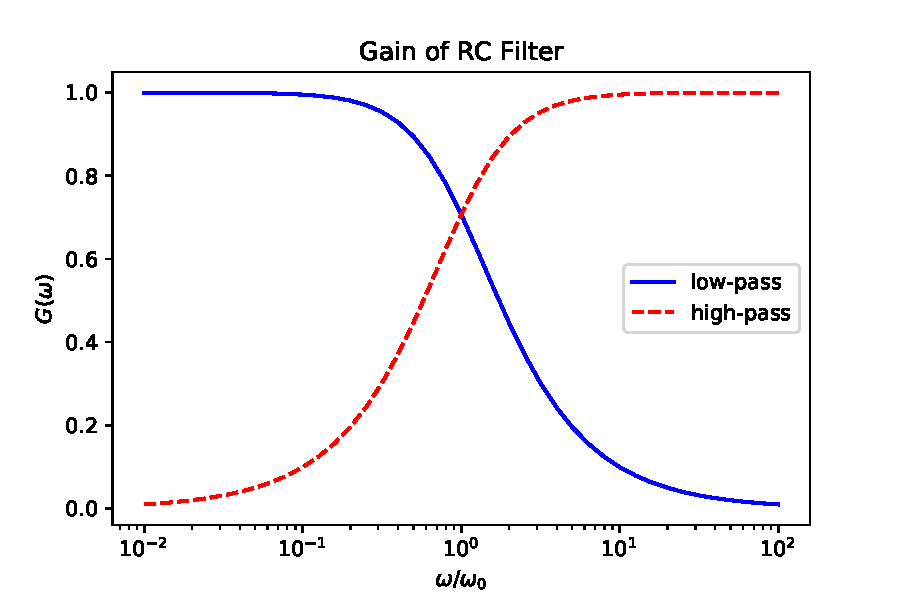
\includegraphics[height=0.3\textheight]{figs/rcgain.pdf} \\
\caption{ The gain of an RC filter.}
\label{fig:rcgain}
\end{center}
\end{figure}
We are particularly interested in the ratio of the output phasor to the input phasor, which defines the complex valued transfer function for the circuit $H(\omega)$:
\begin{equation*}
H(\omega) \equiv \frac{\tilde{v}_{\rm out}}{\tilde{v}_{\rm in}} = \frac{1}{1 + j \omega/\omega_0}\\
\end{equation*}
Our primary concern is generally the ratio of the amplitude of the output voltage to the amplitude of the input voltage, without concern for phase, which we call the gain $G(\omega)$:
\begin{equation*}
G(\omega) \equiv \frac{|\tilde{v}_{\rm out}|}{|\tilde{v}_{\rm in}|} = |H(\omega)| 
\end{equation*}
which is in this case:
\begin{eqnarray*}
G(\omega) &=& |H| = \frac{1}{|1 - j \omega/\omega_0 |}\\
&=& \frac{1}{\sqrt{1+\omega^2/\omega_0^2}}
\end{eqnarray*}
Notice that the gain is a positive real value that depends on the angular frequency $\omega$.
For the filter discussed here, at $\omega=0$, we see that $G=1$, while for $\omega \to \infty$, $G \to 0$.
At the corner frequency $\omega = \omega_0$, we see that $G = 1/\sqrt{2}$.
The function is plotted across five orders of magnitude in Fig.~\ref{fig:rcgain}.
We can see that below the corner frequency, the gain is everywhere nearly one, while above the corner frequency, the gain falls to zero.  Low-pass filters attenuate frequencies below the corner frequency while passing frequencies below the corner frequency unchanged.

It is left as an exercise to show that for the high-pass filter, with the roles of $R$ and $C$ interchanged, the transfer function is:
\begin{equation*}
H(\omega) \equiv \frac{\tilde{v}_{\rm out}}{\tilde{v}_{\rm in}} = \frac{1}{1 - j \omega_0/\omega}\\
\end{equation*}
with the corner angular frequency $\omega_0$ defined as before.  The gain is therefore:
\begin{equation*}
G(\omega) = \frac{1}{\sqrt{1+\omega_0^2/\omega^2}}
\end{equation*}
As shown in Fig.~\ref{fig:rcgain} the response of the high-pass filter is complementary to the low-pass filter:  the high-pass filter tends to reject signals with frequencies below the corner frequency while leaving signals with frequencies above the corner frequency unchanged.

\section{Decibels}

The decibel is an often confusing, yet widely used, system of measurement used to express the ratio of one value to another on a logarithmic scale.  Decibels were originally used to describe relative power in telecommunications systems, where the definition is:
\begin{equation}
dB = 10 \, \log_{10}(P_1 / P_0)
\end{equation}
where $P_1$ is the power we are describing relative to the power $P_0$.  In many system there is a quadratic relation between the power and another quantity, which is called a root-power quantity.
For instance, the power in a resistor is $P=V^2/R$.  When using a root-power quantity such as $V$, the definition of a dB is adjusted by a factor of two:
\begin{equation}
dB = 20 \, \log_{10}(V_1 / V_0)
\end{equation}
This allows us to refer to e.g. the $X$ dB point in a way that is independent of whether we refer to power or amplitude, an advantage of dubious value.

Things tend to get a bit more confusing when we move from using decibels to describe a ratio to describing a single quantity.  In this case, the reference value is added to the unit, e.g. dBV is decibel calculated with respect to a one Volt reference.   The special case of measuring power in milliWatts is given the unit dBm.  It is basically a nightmare of implicit definitions as a work-around for the inconvenient fact that the log function insists on a dimensionless quantity.

If you pick a nice sunny day, and linger outside Kemper hall long enough, you are all but guaranteed to hear someone mention ``the three dB point".   This benchmark point result from the unhappy\footnote{for those of that wish dB did not exist.} coincidence that:
\begin{equation*}
10 \log_{10} 2 = 3.01
\end{equation*}
In an $RC$ filter at the corner frequency with $\omega = \omega_0$, the voltage gain is $1/\sqrt{2}$ and the power gain is $1/2$, so the gain in dB is nearly -3.  For an RC circuit, the corner frequency is the ``negative three dB point.''

Undoubtably one reason the dB persists as a unit is that knowing the negative three dB point and then the easily calculated powers of 10 allows one to estimate the response of a system across a wide range:
\begin{eqnarray*}
20 \log_{10} \frac{1}{\sqrt{2}} &\sim& -3~\rm dB\\
20 \log_{10} \frac{1}{10} &=& -20~\rm dB\\
20 \log_{10} \frac{1}{100} &=& -40~\rm dB\\
\end{eqnarray*}
See Fig.~\ref{fig:rcbode}.

\section{Phase Change in Passive Filters}

So far we've considered only the effect of an $RC$ filter on the magnitude of the voltage.  We've yet to consider the phase.  This phase information is contained in complex valued transfer function:
\begin{displaymath}
H = \frac{\tilde{v}_{\rm out}}{\tilde{v}_{\rm in}} 
\end{displaymath}
The change in phase of the output relative to input is simply the polar coordinate $\phi$ of the complex number $H$:
\begin{displaymath}
\phi(H) = \tan^{-1}\left( \frac{\Im{H}}{\Re{H}}\right)
\end{displaymath}
Which in the case of a low-pass filter, results in the phase change:
\begin{displaymath}
\phi = -\tan^{-1} \left( \frac{\omega}{\omega_0}\right)
\end{displaymath}
and for the high-pass filter:
\begin{displaymath}
\phi = \tan^{-1} \left( \frac{\omega_0}{\omega}\right)
\end{displaymath}
as illustrated in Fig.~\ref{fig:rcbode}.  When considering phase changes, it's useful to consider the following benchmarks:
\begin{eqnarray*}
\tan^{-1}(1)  &=& \frac{\pi}{4} = 45^\circ\\
\tan^{-1}(0.1)  &=& 6^\circ\\
\tan^{-1}(10.0)  &=& 90 - 6^\circ\\
\end{eqnarray*}
So we can see that the phase change at the corner frequency is $45^\circ$ and is within $6^\circ$ of the asymptotic value after 1 order of magnitude in frequency.

\begin{figure}[htbp]
\begin{center}
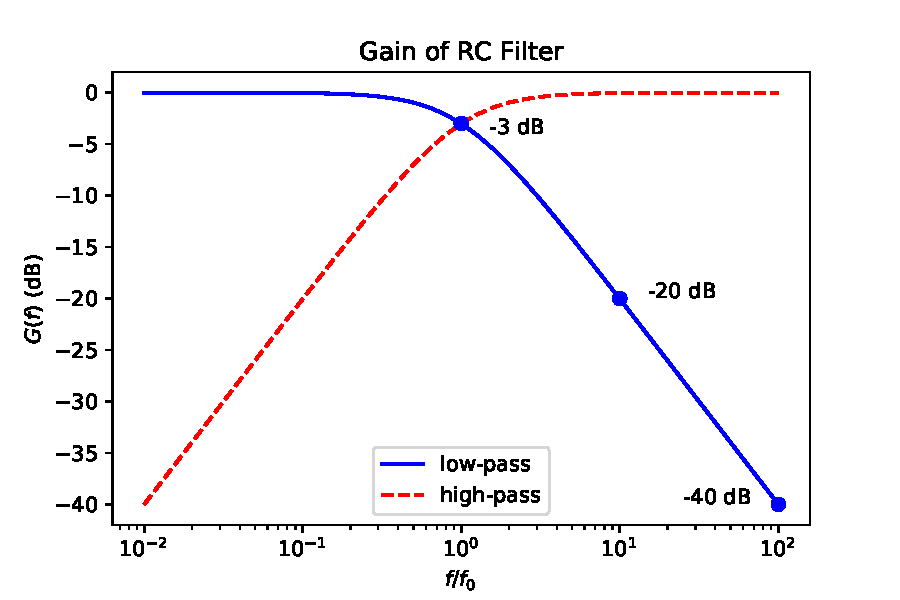
\includegraphics[height=0.3\textheight]{figs/rcgaindb.pdf} \\
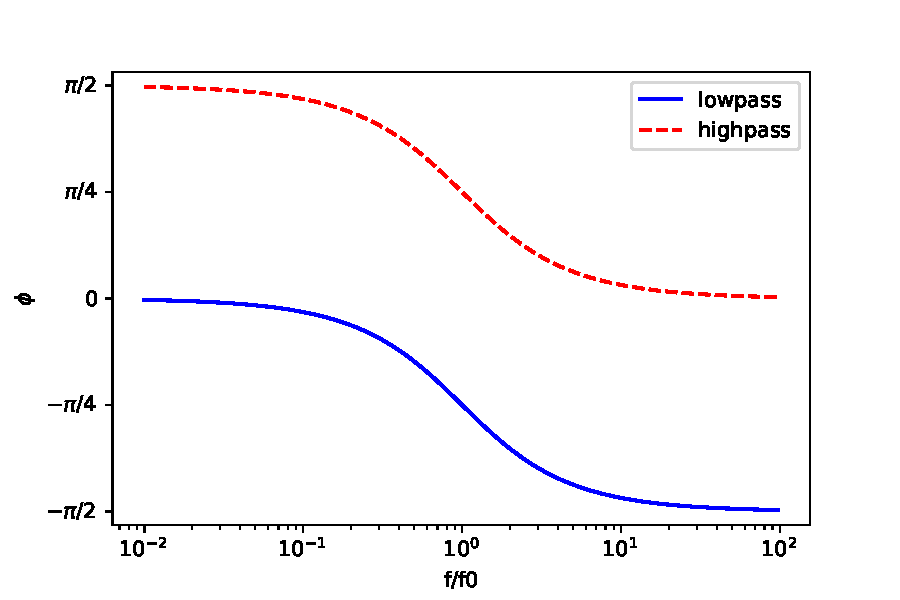
\includegraphics[height=0.3\textheight]{figs/rcphase.pdf} \\
\caption{ The upper plot shows the gain in decibels of an RC filter as a function of frequency, while the lower plot shows the corresponding phase shifts.  Together, these are referred to as the Bode plots for the filter (pronounced ``boh-dee".)}
\label{fig:rcbode}
\end{center}
\end{figure}

\section{Exercises}
\begin{enumerate}
\item Show that for a sinusoidal AC voltage $v_{\rm rms} = v_{\rm p} / \sqrt{2}$.
\item Derive the steady-state solution Equation~\ref{eqn:inductorss} and the general solution Equation~\ref{eqn:inductorgen} for the LR circuit of Fig.~\ref{fig:rl}.


\item Use the impedance formula for capacitors $Z=1/j \omega C $ plus the formulas for equivalent impedance of parallel and series impedances to derive the usual formulas for the equivalent capacitance  of two capacitors in parallel:
\begin{displaymath}
C_{\rm eq} = C_1 + C_2
\end{displaymath}
and in series:
\begin{displaymath}
\frac{1}{C_{\rm eq}} = \frac{1}{C_1} + \frac{1}{C_2}
\end{displaymath}

\item Use the impedance formula for inductors $Z=j \omega L $ plus the formulas for equivalent impedance of parallel and series impedances to derive the usual formulas for the equivalent capacitance  of two inductors in parallel:
\begin{displaymath}
\frac{1}{L_{\rm eq}} = \frac{1}{L_1} + \frac{1}{L_2}
\end{displaymath}
and in series:
\begin{displaymath}
L_{\rm eq} = L_1 + L_2
\end{displaymath}
\item On the complex plane, draw three vectors for the impedance of an inductor, resistor, and capacitor and show that phase factors from Table~\ref{tbl:impedance} can be read directly from plot.
\item Show that you can construct a low-pass and high-pass filter using an inductor and resistor in series and determine the corner angular frequency $\omega_0$ in terms of the inductance $L$ and the resistance $R$.  Note that such filters are rarely used, because real inductors are expensive and generally have more non-ideal characteristics.
\begin{figure}[htbp]
\begin{center}
\begin{circuitikz}[line width=1pt]
\draw (0,0) to[sinusoidal voltage source,bipoles/length=1.5cm] ++(0,3.0) 
to[R,-*,l_=$R$] ++(2.0,0) coordinate(X) to[short,*-*] ++(1.5,0) coordinate(Y) to[short,-o] ++(1.0,0) node[right]{$\tilde{v}_{\rm out}$};
\draw (0.0,2.25) node[left]{$\tilde{v}_{\rm in}$};
\draw (X) to[C,-*,l=$C$] ++(0,-3.0)  to[short,-*] ++(-2.0,0) node[ground,yscale=2.0]{};
\draw (Y) to[L,-*,l=$L$] ++(0,-3.0)  coordinate(X) to[short,-*] ++(-1.5,0);
%\draw (X) to[short,-o] ++(1.0,0) node[right]{A};
\end{circuitikz}  
\caption{A function generator driving a resistor.}
\label{fig:rlccircuit}
\end{center}
\end{figure}
\item Consider the RLC filter of Fig.~\ref{fig:rlccircuit}.  Derive the transfer function for the circuit and find the resonant angular frequency $\omega_0$ for which the gain is 1.
\end{enumerate}

\chapter{The Diode}

\section{Semiconductors}

\begin{figure}[htbp]
\begin{center}
\begin{tikzpicture}
%\draw[step=1cm,gray,very thin] (0,0) grid (12,5);
\draw (1,1) circle (0.5cm) node{A};
\draw (11,1) circle (0.5cm) node{B};
\draw (5.5,1) circle (0.5cm) node{A};
\draw (6.5,1) circle (0.5cm) node{B};
\draw (0,3) -- ++(2,0);
\draw (10,3) -- ++(2,0);
\draw (5,2) -- ++(2,0);
\draw (5,4) -- ++(2,0);
\draw[dashed] (2,3) -- (5,2);
\draw[dashed] (2,3) -- (5,4);
\draw[dashed] (10,3) -- (7,2);
\draw[dashed] (10,3) -- (7,4);
\draw[thick,->] (0.5,3) -- ++(0,0.5);
\draw[thick,<-] (10.5,3) -- ++(0,0.5);
\draw[thick,->] (5.5,2) -- ++(0,0.5);
\draw[thick,<-] (6.5,2) -- ++(0,0.5);
%\node at (1,1) {A};
\end{tikzpicture}
\caption{When two identical atoms A and B are brought close together, the two degenerate energy eigenstates for an electron (located at atom A or B) are replaced with two states of differing energy, equally shared between atoms A and B.}
\label{fig:bond}
\end{center}
\end{figure}

Consider the simple quantum mechanical model illustrated in Fig.~\ref{fig:bond}.  When two identical atoms, A and B, are very far apart, they can be considered separately, and the energy eigenstates are degenerate in energy.  For each solution for an electron located at atom A, there is a solution of equal energy for an electron located at atom B.  When the atoms A and B are brought close enough together, a particle located at atom A can quantum mechanically tunnel to atom B, and so these states are no longer energy eigenstates.  Instead, the eigenstates share the electron equally between A and B, in either a symmetric or antisymmetric wave function.  The symmetric wave function has lower energy than the antisymmetric wave function, so that the energy levels are no longer degenerate.  If the outer most level is not full, this results in a lower total energy through sharing, which is the quantum mechanical explanation for a covalent bond.

\begin{figure}[htbp]
\begin{center}
\begin{tikzpicture}
\draw (0,3) -- ++(1,0);
\draw (2,4) -- ++(1,0);
\draw (2,2) -- ++(1,0);
\draw (4,4.5) -- ++(1,0);
\draw (4,3.5) -- ++(1,0);
\draw (4,2.5) -- ++(1,0);
\draw (4,1.5) -- ++(1,0);
\draw (6,1.0) -- ++(1,0);
\draw (6,1.5) -- ++(1,0);
\draw (6,2.0) -- ++(1,0);
\draw (6,2.5) -- ++(1,0);
\draw (6,3.0) -- ++(1,0);
\draw (6,3.5) -- ++(1,0);
\draw (6,4.0) -- ++(1,0);
\draw (6,4.5) -- ++(1,0);
\draw (6,5.0) -- ++(1,0);
\node at (0.5,0.5) {$n=1$};
\node at (2.5,0.5) {$2$};
\node at (4.5,0.5) {$4$};
\node at (6.5,0.5) {$8$};
\node at (8.5,0.5) {$10^{23}$};
\draw[thick] (8,0.75) rectangle (9,5.25);
\end{tikzpicture}
\caption{As more and more identical atoms are brought close together, the number of distinct energy levels increases until there is an effectively continuous band of available energies.}
\label{fig:bands}
\end{center}
\end{figure}

\begin{figure}[htbp]
\begin{center}
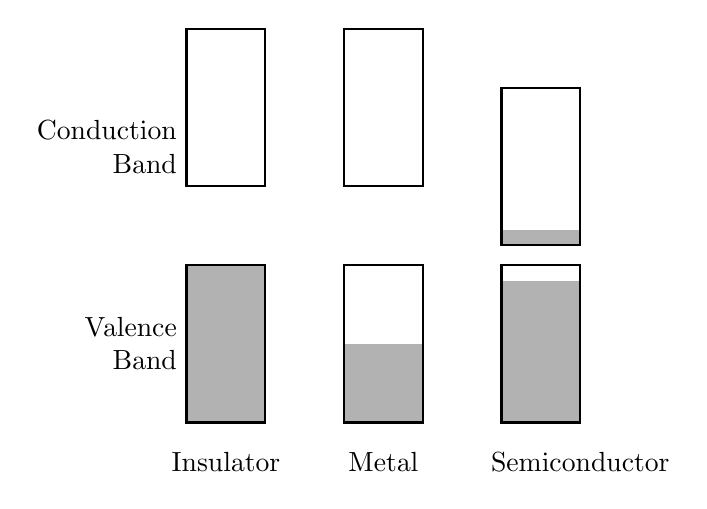
\begin{tikzpicture}
%\draw[step=1cm,gray,very thin] (0,0) grid (6,6);
\fill[black!30!white] (0,1) rectangle ++(1,2);
\draw[thick] (0,1) rectangle ++(1,2);
\draw[thick] (0,4) rectangle ++(1,2);
\fill[black!30!white] (2,1) rectangle ++(1,1);
\draw[thick] (2,1) rectangle ++(1,2);
\draw[thick] (2,4) rectangle ++(1,2);
\fill[black!30!white] (4,1) rectangle ++(1,1.8);
\fill[black!30!white] (4,3.25) rectangle ++(1,0.2);
\draw[thick] (4,1) rectangle ++(1,2);
\draw[thick] (4,3.25) rectangle ++(1,2);
\node[left, align=right] at (0,4.5) {Conduction \\ Band};
\node[left, align=right] at (0,2) {Valence \\Band};
\node at (0.5,0.5) {Insulator};
\node at (2.5,0.5) {Metal};
\node at (5.0,0.5) {Semiconductor};
\end{tikzpicture}
\caption{The valance and conduction bands for insulators, metals, and semiconductor.  The shared regions indicate electrons}
\label{fig:materials}
\end{center}
\end{figure}




Now consider what happens when an Avagadro's number ($\sim 10^{23}$) of molecules or atoms are brought together to form a periodic lattice.  As illustrated in Fig.~\ref{fig:bands} each discrete energy level in the single atom is replaced by a nearly continuous band of available energies in the lattice.  Many of the important properties of materials can be understood by considering only the energy band that contains the highest energy electron (called the valance band) and the band directly above it (called the conduction band).  

As shown in Fig.~\ref{fig:materials}, an insulator consists of a full valence band separated from the conduction band by a large gap.  The complete set of possible wave functions for an electron in the valance band can be though of as left-traveling and right-traveling waves.  From symmetry there are an equal number of left and right traveling waves.  When a band is full, there are therefore always an equal number of left and right traveling waves and no net current.  A metal has a partially full valance band, and therefore no difficulty conducting charge.

A semiconductor contains a full valance band separated from the conductor by a small band gap.  As a result, thermal fluctuations allow electrons in the valance band to gain sufficient energy to enter the conduction band, leaving an unfilled state in the valance band.  The electrons in the conduction band can conduct electricity.  The vacant states in the valance band can also conduct electricity, as the absence of a negative charge acts like a mobile positive charge, which is called a hole.

Intrinsic semiconductors have an equal number of electrons and holes.  However, in a process called doping, different molecules are added periodically to the semiconductor lattice that tend to provide additional electrons to the conduction material or absorb additional electrons from the valance band.  This leads to either an excess of holes in $p$-type semiconductors and an excess in electrons in $n$-type semiconductors.  Semiconductors are the core technology upon which the entire modern electronics industry is based.

\section{The Diode}

\begin{figure}[htbp]
\begin{center}
\begin{tabular}{cc}
\begin{circuitikz}[line width=1pt]
%\draw (0,0) to[voltage source,bipoles/length=1.5cm,l=$V$] ++(0,+3.0) to[D] ++(3.0,0);
\draw(0,0) to[D] ++(3,0);
\end{circuitikz} &
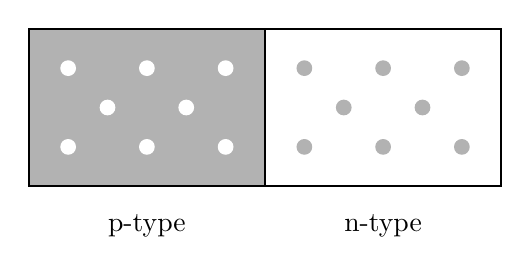
\begin{tikzpicture}
%\draw[step=1cm,gray,very thin] (0,0) grid (6,3);
\fill[black!30!white] (0,1) rectangle ++(3,2);
\draw[thick] (0,1) rectangle ++(3,2);
\draw[thick] (3,1) rectangle ++(3,2);
\fill[white] (0.5,1.5) circle (0.10);
\fill[white] (0.5,2.5) circle (0.10);
\fill[white] (1.5,1.5) circle (0.10);
\fill[white] (1.5,2.5) circle (0.10);
\fill[white] (2.5,1.5) circle (0.10);
\fill[white] (2.5,2.5) circle (0.10);
\fill[white] (1,2) circle (0.10);
\fill[white] (2,2) circle (0.10);
\fill[black!30!white] (3.5,1.5) circle (0.10);
\fill[black!30!white] (3.5,2.5) circle (0.10);
\fill[black!30!white] (4.5,1.5) circle (0.10);
\fill[black!30!white] (4.5,2.5) circle (0.10);
\fill[black!30!white] (5.5,1.5) circle (0.10);
\fill[black!30!white] (5.5,2.5) circle (0.10);
\fill[black!30!white] (4,2) circle (0.10);
\fill[black!30!white] (5,2) circle (0.10);
\node at (1.5,0.5) {p-type};
\node at (4.5,0.5) {n-type};
\end{tikzpicture}
\\
(a)&
(b)\\
\end{tabular}
\caption{The diode (a) circuit diagram, and (b) as a junction between p-type and n-type semiconductor.  The white circles represent holes and the gray circles represent electrons.}
\label{fig:diode}
\end{center}
\end{figure}

\begin{figure}[htbp]
\begin{center}
\begin{tabular}{cc}
\begin{circuitikz}[line width=1pt]
\draw (0,0) to[short,i<=$I$] ++(0,+3.0) to[D] ++(3.0,0);
\draw (0,0) to[short] ++(3,0) to[voltage source,bipoles/length=1.5cm] ++(0,3);
\end{circuitikz} &
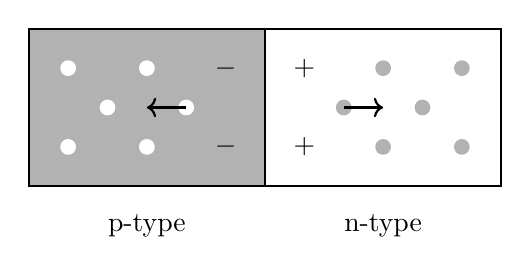
\begin{tikzpicture}
%\draw[step=1cm,gray,very thin] (0,0) grid (6,3);
\fill[black!30!white] (0,1) rectangle ++(3,2);
\draw[thick] (0,1) rectangle ++(3,2);
\draw[thick] (3,1) rectangle ++(3,2);
\fill[white] (0.5,1.5) circle (0.10);
\fill[white] (0.5,2.5) circle (0.10);
\fill[white] (1.5,1.5) circle (0.10);
\fill[white] (1.5,2.5) circle (0.10);
%\fill[white] (2.5,1.5) circle (0.10);
%\fill[white] (2.5,2.5) circle (0.10);
\node at (2.5,1.5) {$-$};
\node at (2.5,2.5) {$-$};
\fill[white] (1,2) circle (0.10);
\fill[white] (2,2) circle (0.10);
%\fill[black!30!white] (3.5,1.5) circle (0.10);
%\fill[black!30!white] (3.5,2.5) circle (0.10);
\node at (3.5,1.5) {$+$};
\node at (3.5,2.5) {$+$};
\fill[black!30!white] (4.5,1.5) circle (0.10);
\fill[black!30!white] (4.5,2.5) circle (0.10);
\fill[black!30!white] (5.5,1.5) circle (0.10);
\fill[black!30!white] (5.5,2.5) circle (0.10);
\fill[black!30!white] (4,2) circle (0.10);
\fill[black!30!white] (5,2) circle (0.10);
\draw[thick,->] (4,2) -- ++(0.5,0);
\draw[thick,->] (2,2) -- ++(-0.5,0);
\node at (1.5,0.5) {p-type};
\node at (4.5,0.5) {n-type};
\end{tikzpicture}
\\
(a)&
(b)\\
\end{tabular}
\caption{The diode is in reverse bias when the (a) the applied voltage directs a positive current through the diode opposite the arrow in the diode diagram, and (b) which tends to pull mobile holes and electrons away from the p-n junction, creating a depletion zone.}
\label{fig:dioderev}
\end{center}
\end{figure}


\begin{figure}[htbp]
\begin{center}
\begin{tabular}{cc}
\begin{circuitikz}[line width=1pt]
\draw (0,0) to[voltage source,bipoles/length=1.5cm,i>=$I$] ++(0,+3.0) to[D] ++(3.0,0) |- (0,0);
\end{circuitikz} &
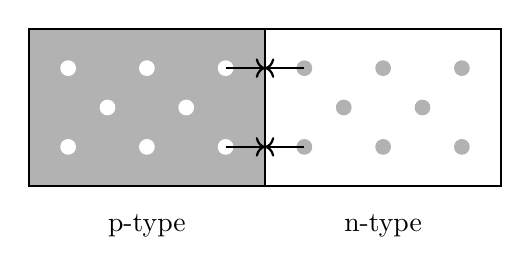
\begin{tikzpicture}
%\draw[step=1cm,gray,very thin] (0,0) grid (6,3);
\fill[black!30!white] (0,1) rectangle ++(3,2);
\draw[thick] (0,1) rectangle ++(3,2);
\draw[thick] (3,1) rectangle ++(3,2);
\fill[white] (0.5,1.5) circle (0.10);
\fill[white] (0.5,2.5) circle (0.10);
\fill[white] (1.5,1.5) circle (0.10);
\fill[white] (1.5,2.5) circle (0.10);
\fill[white] (2.5,1.5) circle (0.10);
\fill[white] (2.5,2.5) circle (0.10);
\fill[white] (1,2) circle (0.10);
\fill[white] (2,2) circle (0.10);
\fill[black!30!white] (3.5,1.5) circle (0.10);
\fill[black!30!white] (3.5,2.5) circle (0.10);
\fill[black!30!white] (4.5,1.5) circle (0.10);
\fill[black!30!white] (4.5,2.5) circle (0.10);
\fill[black!30!white] (5.5,1.5) circle (0.10);
\fill[black!30!white] (5.5,2.5) circle (0.10);
\fill[black!30!white] (4,2) circle (0.10);
\fill[black!30!white] (5,2) circle (0.10);
\node at (1.5,0.5) {p-type};
\node at (4.5,0.5) {n-type};
\draw[thick,->] (2.5,1.5) -- (3.0,1.5);
\draw[thick,->] (2.5,2.5) -- (3.0,2.5);
\draw[thick,->] (3.5,1.5) -- (3.0,1.5);
\draw[thick,->] (3.5,2.5) -- (3.0,2.5);
\end{tikzpicture}
\\
(a)&
(b)\\
\end{tabular}
\caption{The diode is in forward bias when the (a) applied voltage directs a positive current in the same direction as the arrow in the diode symbol, and (b) tends to move electrons and holes toward the pn junction, where they recombine. }
\label{fig:diodefwd}
\end{center}
\end{figure}

A diode is a junction of $p$-type and $n$-type semiconductor as shown in Fig.~\ref{fig:diode}.   The diode has an interesting and useful $V$-$I$ curve that depends on the polarity of the applied voltage.  Consider first what happens if we apply a reverse-bias voltage as illustrated in Fig.~\ref{fig:dioderev}.  In this configuration, the applied voltage initially creates a current which move holes to left and electrons to right, which in both cases moves the mobile charge carriers away from the pn junction.  This creates a depletion zone at the junction with no mobile charge carriers.  Because the semiconductors initially had no net charge, as holes move out of the depletion zone in the p-type semiconductor, they leave behind a fixed negative charge.  Likewise, as electrons move out of the depletion zone in the n-type semiconductor, the leave behind a fixed positive charge.  The fixed charges create an electric field which results in a voltage across the depletion zone.  The depletion zone widens until the voltage across the depletion zone equals the applied voltage, at which point no current flows.  In the steady-state, a diode in reverse bias passes no current.  

Now consider what happens if we apply a forward-bias voltage as illustrated in Fig.~\ref{fig:dioderev}.  In this configuration, the applied voltage produces a current which moves holes to right and electrons to the left, which in both cases moves the mobile charge carriers toward the pn junction.  At this junction, the electrons recombine with holes, which allows a current in this direction to continue as long as the voltage is applied.


\begin{figure}[htbp]
\begin{center}
\begin{tabular}{p{2cm}p{2cm}p{2cm}c}
\begin{circuitikz}[line width=1pt]
\draw(0,0) to[D] ++(0,-3);
\end{circuitikz} &
\begin{circuitikz}[line width=1pt]
\draw(0,0) to[short,-o] ++(0,1);
\draw(0,2) to[short,o-] ++(0,1);
\end{circuitikz} &
\begin{circuitikz}[line width=1pt]
\draw(0,0) to[voltage source,bipoles/length=1.5cm,l=$V_{\rm d}$] ++(0,3);
\end{circuitikz} &
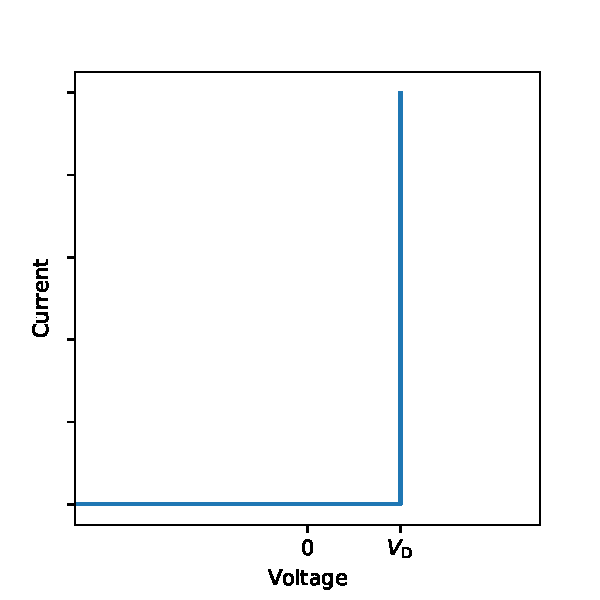
\includegraphics[width=0.45\textwidth]{figs/diodeop.pdf} \\
(a) & (b) & (c) & (d) \\
\end{tabular}
\caption{Circuit diagram from a (a) diode, equivalent circuits for (b) reverse bias and (c) forward bias, and   the corresponding (d) IV curve.  For a typical silicon diode $V_{\rm D}$ is between $0.6$ and $0.7~\rm V$.}
\label{fig:diodeeqv}
\end{center}
\end{figure}

A diode, therefore, has the very useful feature that it only allows current to flow in one direction.  As shown in Fig.~\ref{fig:diodeeqv} under reverse-bias the diode is equivalent to an open circuit.  Our discussion so far might lead you to think that under forward-bias, the diode is equivalent to a short circuit.  The situation is in fact slightly more complicated.  Absent any applied voltage, thermal fluctuations cause electrons and holes to bump into each other and combine at the pn junction, which causes a small depletion zone to form.   Meanwhile, thermal fluctuations also cause electrons in the valence band to reach the conduction band, creating electron-hole pairs.  The depletion zone increases until an equilibrium is reached between recombination and pair production.  This intrinsic depletion zone is effectively an voltage drop that must be overcome before any current can flow.  The equivalent circuit for a diode in forward bias is therefore a small voltage drop $V_{\rm d}$ as shown in Fig.~\ref{fig:diodeeqv}.  For typical silicon diodes, $V_{\rm d}$ is $0.6$ to $0.7~\rm V$.  Note that the direction of the allowed current in the diode assures us that the diode always consumes power.  It is a passive component and cannot be used to add power to a circuit.

\section{Current Rectification}

\begin{figure}[htbp]
\begin{center}
\begin{tabular}{cc}
\begin{circuitikz}[line width=1pt]
\draw (0,0) node[ground,yscale=2.0]{} to[sinusoidal voltage source,bipoles/length=1.5cm] ++(0,+3.0) 
to[D] ++(3.0,0) coordinate(X) to[R,l=$R_{\rm L}$] ++(0,-3) to[short,-*] ++(-3,0);
\draw (X) to[short,*-o] ++(0.75,0) node[right]{$v_{\rm R}(t)$};
\draw (0.0,2.2) node[left]{$v_{\rm S}(t)$};
\end{circuitikz} &
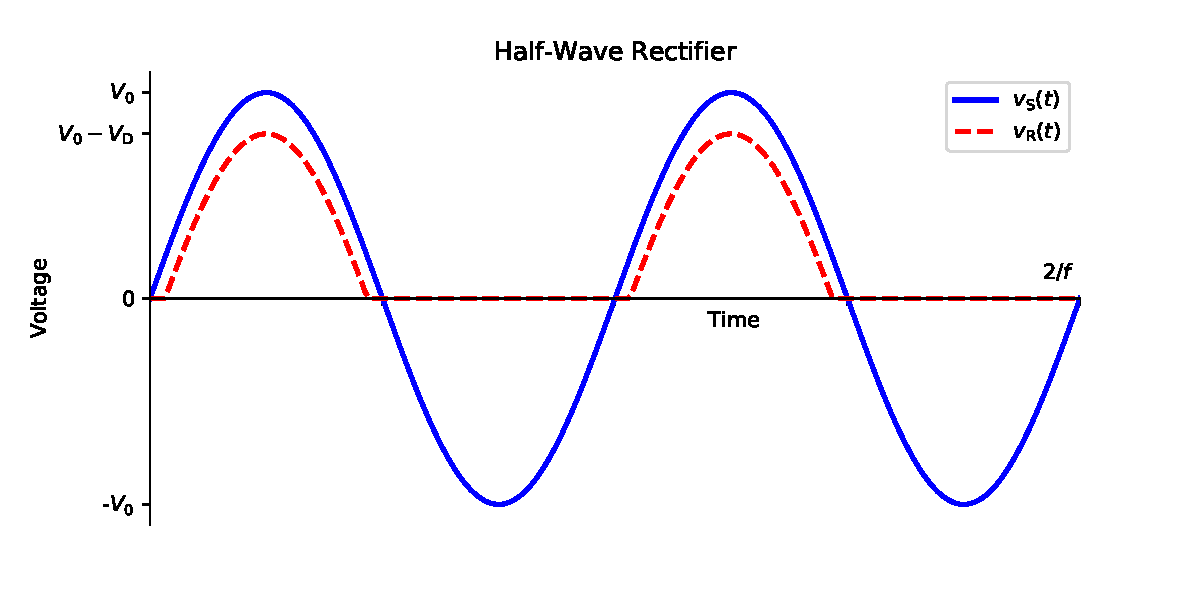
\includegraphics[width=0.55\textwidth]{figs/rectification.pdf} 
\\
(a) & (b) \\
\end{tabular}
\caption{ Half-wave rectifier}
\label{fig:basicrect}
\end{center}
\end{figure}

In the previous section, we discussed that operationally, a diode is an open circuit under reverse bias, and  a constant voltage drop $V_D$ under forward bias.  The IV curve for this operational model of the diode shown in Fig.~\ref{fig:diodeeqv} is usually sufficient for understanding the behavior of circuits involving diodes.  The rectification feature of a diode is illustrated in Fig.~\ref{fig:basicrect}.  The voltage across the resistor is the positive half of the source AC voltage, reduced by one diode drop.

\begin{figure}[htbp]
\begin{center}
\begin{tabular}{cc}
\begin{circuitikz}[line width=1pt]
\draw (0,0) node[ground,yscale=2.0]{} to[sinusoidal voltage source,bipoles/length=1.5cm] ++(0,+3.0) 
to[D] ++(2.0,0) coordinate(X) to[C,l=$C$] ++(0,-3) to[short,-*] ++(-2,0);
\draw (X) to[short,*-] ++(1.0,0) coordinate(X) to[R,l=$R_{\rm L}$] ++(0,-3) to[short,-*] ++(-1,0);
\draw (X) to[short,*-o] ++(0.75,0) node[right]{$v_{\rm R}(t)$};
\draw (0.0,2.2) node[left]{$v_{\rm S}(t)$};
\end{circuitikz} &
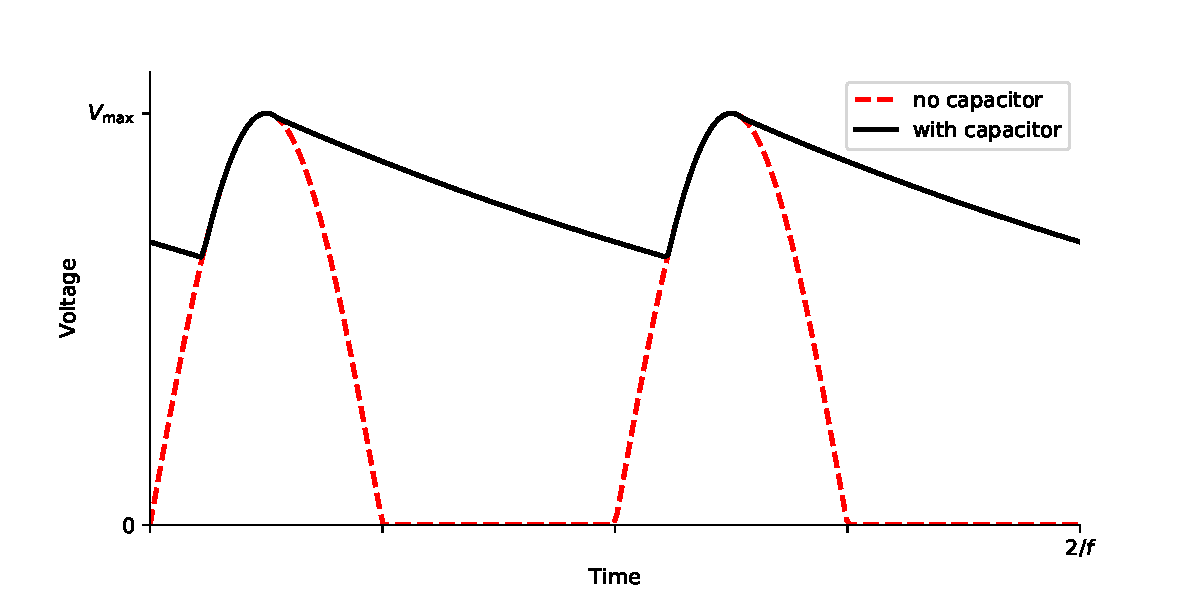
\includegraphics[width=0.55\textwidth]{figs/ripple.pdf} 
\\
(a) & (b) \\
\end{tabular}
\caption{ Half-wave rectifier with capacitor.}
\label{fig:ripple}
\end{center}
\end{figure}

The voltage across the resistor $R_{\rm L}$ (and corresponding current) for the half-wave rectifier circuit in Fig.~\ref{fig:basic} has a non-zero DC component, but it varies significantly as a function of time.  To produce a more constant DC voltage, a capacitor can be used as in Fig.~\ref{fig:ripple}.  The capacitor provides current to the load during the portion of the cycle when the rectified AC voltage is too low.
As the capacitor provides current to the load, it's voltage sags, resulting in AC ripple current in addition to the DC voltage.  The ripple current can be reduced by increasing the size of the capacitor.  We can estimate the size of the ripple current by considering that the voltage sag $\Delta v$ is given by:
\begin{displaymath}
\Delta v = \frac{\Delta q}{C}.
\end{displaymath}
Meanwhile, the most the capacitor can discharge during the cycle of frequency $f=1/T$ is:
\begin{displaymath}
\Delta q = I_{\rm max} \, T = \frac{I_{\rm max}}{f}  
\end{displaymath}
And so the voltage sag is:
\begin{displaymath}
\Delta v = \frac{I_{\rm max}}{fC} = \frac{V_{\rm max}}{fRC}.
\end{displaymath}

\section{Real Diodes}

\begin{figure}[htbp]
\begin{center}
\begin{tabular}{cc}
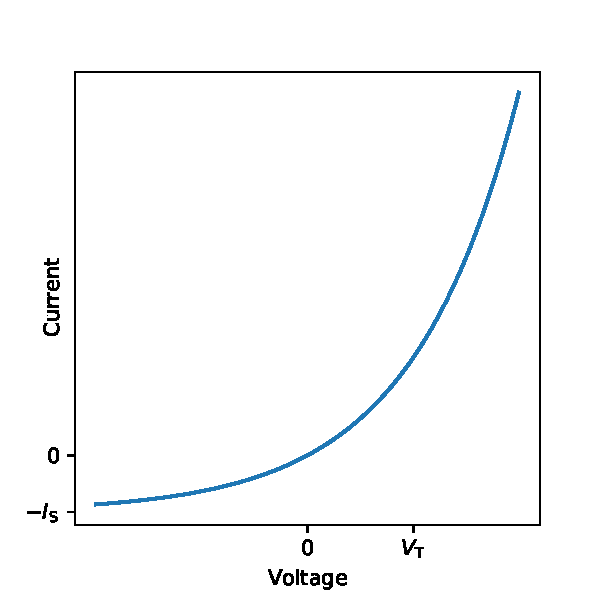
\includegraphics[width=0.45\textwidth]{figs/diodeeq.pdf} &
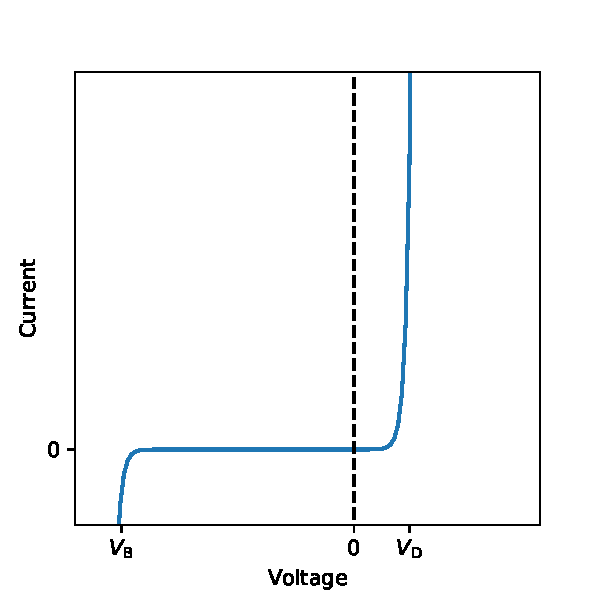
\includegraphics[width=0.45\textwidth]{figs/breakdown.pdf} \\
(a) &
(b) \\
\end{tabular}
\caption{Diode $I$-$V$ curve (a) from the Schockley equations, and (b) from the Schockley equations at wider scale and including breakdown.  Typical values of $V_{\rm T} = 26~\rm mV$, $I_{\rm S} = 5~\rm \mu A$, $V_{\rm D}=0.6~\rm V$}
\label{fig:diodeeqs}
\end{center}
\end{figure}

The useful operational model of the diode differs from real diodes in several ways.  While under reverse bias, thermal fluctuations in the depletion band of diode produce a small but constant supply of mobile charge carriers, which allows a small current to flow under reverse bias.  This current, called the saturation current $I_{\rm S}$ is quite small.  For the 1N914 diode, $I_{\rm S} = 5~\rm \mu A$.
If the reverse bias voltage is increased sufficiently, the small number of mobile charge carriers forming the saturation current are accelerated enough to produce additional electron-hole pairs through collisions, creating a cascade that dramatically increases the reverse current.   Diodes typically have a breakdown voltage below which they will conduct in reverse-bias.  Instead of avalanche breakdown, some diodes breakdown due to quantum tunnelng, by an effect called Zener breakdown.  Zener diodes are specifically designed to provide a nearly constant voltage under reverse bias, and are often used to regulate DC voltage levels.

A full thermodynamic treatment of the pn junction in a diode yields the Schockley diode equation:
\begin{displaymath}
I(V) = I_{\rm S} \left( \exp\left( \frac{V}{V_{\rm T}}\right) - 1 \right)
\end{displaymath}
where $V_{\rm T}$ is the thermal voltage, defined by 
\begin{displaymath}
V_{\rm T} = \frac{kT}{e},
\end{displaymath}
which has the value $26~\rm mV$ at room temperature.  The diode equation is plotted in Fig.~\ref{fig:diodeeqs}a at a scale where the exponential behavior and reverse current are visible.  In Fig.~\ref{fig:diodeeqs}b the scale is adjusted to typical scale for circuit parameters, and the curve much more closely resembles the simple operational model. 

\end{document}




